% Build with XeLaTeX; see README.md for fonts and commands.
\documentclass[12pt,a4paper]{report}

% =========================================================================
% GOI THU VIEN & CAU HINH CO BAN -- giu phong cach Assignment 01
% =========================================================================
\usepackage{iftex}
\ifPDFTeX
    \usepackage[utf8]{inputenc}
    \usepackage[T5]{fontenc}
    \usepackage[vietnamese]{babel}
    \usepackage{newtxtext}
\else
    \usepackage{fontspec}
    \defaultfontfeatures{Ligatures=TeX}
    \IfFontExistsTF{Times New Roman}
        {\setmainfont{Times New Roman}}
        {\setmainfont{TeX Gyre Termes}}
\fi

\usepackage[top=2.5cm,bottom=2.5cm,left=3.0cm,right=2.0cm]{geometry}
\usepackage{amsmath,amsfonts,amssymb}
\ifPDFTeX
    \usepackage{newtxmath}
\fi
\usepackage{graphicx}
\usepackage{booktabs}
\usepackage{tabularx}
\usepackage{multirow}
\usepackage{array}
\usepackage{float}
\usepackage{needspace}
\usepackage{xcolor}
\usepackage{tikz}
\usetikzlibrary{calc,shapes.geometric,arrows,positioning,arrows.meta}
\usepackage{fancyhdr}
\usepackage{titlesec}
\usepackage{caption}
\usepackage{subcaption}
\usepackage{enumitem}
\usepackage{listings}
\usepackage{textcomp}
\usepackage{hyperref}

\newcommand{\missinggraphic}[1]{%
    \begingroup
    \setlength{\fboxsep}{6pt}%
    \fbox{\parbox[c][2.4cm][c]{0.82\linewidth}{%
        \centering\footnotesize Chưa có ảnh\\[2pt]
        \texttt{\detokenize{#1}}% 
    }}%
    \endgroup
}
\newcommand{\safeincludegraphics}[2][]{%
    \IfFileExists{#2}{\includegraphics[#1]{#2}}{\missinggraphic{#2}}%
}
\newcommand{\sourcecodefigure}[3]{%
    \begin{figure}[H]
        \centering
        \safeincludegraphics[width=0.96\textwidth]{#1}
        \caption{#2}
        \label{#3}
    \end{figure}
}
\newcommand{\analysisblock}[3]{%
    \noindent\textbf{Quan sát.} #1\par
    \noindent\textbf{Diễn giải.} #2\par
    \noindent\textbf{Hàm ý đối với ML.} #3\par
}
\newcolumntype{Y}{>{\raggedright\arraybackslash}X}
\newcolumntype{C}[1]{>{\centering\arraybackslash}p{#1}}

\hypersetup{
    unicode=true,
    colorlinks=true,
    allcolors=black,
    pdftitle={Project01 Diabetes Agent},
    pdfauthor={Bùi Anh Đức - B23DCCN165}
}
\urlstyle{same}
\setlength{\emergencystretch}{2em}

\definecolor{codegreen}{rgb}{0,0.6,0}
\definecolor{codegray}{rgb}{0.5,0.5,0.5}
\definecolor{codepurple}{rgb}{0.58,0,0.82}
\definecolor{backcolour}{rgb}{0.96,0.97,0.98}
\lstdefinestyle{mystyle}{
    backgroundcolor=\color{backcolour},
    commentstyle=\color{codegreen},
    keywordstyle=\color{blue!80!black}\bfseries,
    numberstyle=\tiny\color{codegray},
    stringstyle=\color{codepurple},
    basicstyle=\ttfamily\footnotesize,
    breakatwhitespace=false,
    breaklines=true,
    captionpos=b,
    keepspaces=true,
    numbers=left,
    numbersep=5pt,
    showspaces=false,
    showstringspaces=false,
    showtabs=false,
    tabsize=2,
    frame=single,
    rulecolor=\color{black!20}
}
\lstset{style=mystyle}
\ifPDFTeX\else
\IfFontExistsTF{Consolas}{\setmonofont{Consolas}[Scale=MatchLowercase]}{\setmonofont{DejaVu Sans Mono}[Scale=MatchLowercase]}
\fi
\lstdefinestyle{projectcode}{style=mystyle,language=Python,
  basicstyle=\ttfamily\fontsize{9}{11}\selectfont,
  numberstyle=\ttfamily\fontsize{7}{9}\selectfont\color{codegray},
  columns=fullflexible,breaklines=true,breakatwhitespace=false,upquote=true,
  xleftmargin=15pt,xrightmargin=3pt,framexleftmargin=3pt,
  aboveskip=7pt,belowskip=10pt,captionpos=b}
\ifPDFTeX\else
\makeatletter
\begingroup\catcode0=12\relax
\gdef\reportunicode{\lst@CCECUse\lst@ProcessLetter Đđơưạảấầẫậắằẵặếềểệịốồổỗộờợụứửữự^^00}
\endgroup
\lst@AddToHook{SelectCharTable}{\reportunicode}
\makeatother
\fi
\newcommand{\reportcode}[2]{\csname code@#1\endcsname{#2}}
\expandafter\def\csname code@data_check\endcsname#1{%
\par\noindent\begin{minipage}{\linewidth}
\noindent{\footnotesize\textit{Nguồn: }\path{diabetes_agent/data.py}, dòng 11--26.}\par\smallskip
\lstinputlisting[style=projectcode,firstnumber=11,gobble=0,caption={#1}]{snippets/data_check.py}
\end{minipage}\par}
\expandafter\def\csname code@architecture\endcsname#1{%
\par\noindent\begin{minipage}{\linewidth}
\noindent{\footnotesize\textit{Nguồn: }\path{diabetes_agent/models.py}, dòng 28--30.}\par\smallskip
\lstinputlisting[style=projectcode,firstnumber=28,gobble=0,caption={#1}]{snippets/architecture.py}
\end{minipage}\par}
\expandafter\def\csname code@train_setup\endcsname#1{%
\par\noindent\begin{minipage}{\linewidth}
\noindent{\footnotesize\textit{Nguồn: }\path{diabetes_agent/models.py}, dòng 78--88.}\par\smallskip
\lstinputlisting[style=projectcode,firstnumber=78,gobble=4,caption={#1}]{snippets/train_setup.py}
\end{minipage}\par}
\expandafter\def\csname code@train_loop\endcsname#1{%
\par\noindent\begin{minipage}{\linewidth}
\noindent{\footnotesize\textit{Nguồn: }\path{diabetes_agent/models.py}, dòng 89--113.}\par\smallskip
\lstinputlisting[style=projectcode,firstnumber=89,gobble=4,caption={#1}]{snippets/train_loop.py}
\end{minipage}\par}
\expandafter\def\csname code@threshold\endcsname#1{%
\par\noindent\begin{minipage}{\linewidth}
\noindent{\footnotesize\textit{Nguồn: }\path{diabetes_agent/models.py}, dòng 33--36.}\par\smallskip
\lstinputlisting[style=projectcode,firstnumber=33,gobble=0,caption={#1}]{snippets/threshold.py}
\end{minipage}\par}
\expandafter\def\csname code@model_selection\endcsname#1{%
\par\noindent\begin{minipage}{\linewidth}
\noindent{\footnotesize\textit{Nguồn: }\path{diabetes_agent/models.py}, dòng 133--145.}\par\smallskip
\lstinputlisting[style=projectcode,firstnumber=133,gobble=4,caption={#1}]{snippets/model_selection.py}
\end{minipage}\par}
\expandafter\def\csname code@inference\endcsname#1{%
\par\noindent\begin{minipage}{\linewidth}
\noindent{\footnotesize\textit{Nguồn: }\path{diabetes_agent/models.py}, dòng 178--193.}\par\smallskip
\lstinputlisting[style=projectcode,firstnumber=178,gobble=4,caption={#1}]{snippets/inference.py}
\end{minipage}\par}
\expandafter\def\csname code@retrieval\endcsname#1{%
\par\noindent\begin{minipage}{\linewidth}
\noindent{\footnotesize\textit{Nguồn: }\path{diabetes_agent/knowledge.py}, dòng 26--53.}\par\smallskip
\lstinputlisting[style=projectcode,firstnumber=26,gobble=4,caption={#1}]{snippets/retrieval.py}
\end{minipage}\par}
\expandafter\def\csname code@q_learning\endcsname#1{%
\par\noindent\begin{minipage}{\linewidth}
\noindent{\footnotesize\textit{Nguồn: }\path{diabetes_agent/rl.py}, dòng 26--40.}\par\smallskip
\lstinputlisting[style=projectcode,firstnumber=26,gobble=0,caption={#1}]{snippets/q_learning.py}
\end{minipage}\par}
\expandafter\def\csname code@message_bus\endcsname#1{%
\par\noindent\begin{minipage}{\linewidth}
\noindent{\footnotesize\textit{Nguồn: }\path{diabetes_agent/system.py}, dòng 70--81.}\par\smallskip
\lstinputlisting[style=projectcode,firstnumber=70,gobble=4,caption={#1}]{snippets/message_bus.py}
\end{minipage}\par}
\expandafter\def\csname code@council\endcsname#1{%
\par\noindent\begin{minipage}{\linewidth}
\noindent{\footnotesize\textit{Nguồn: }\path{diabetes_agent/system.py}, dòng 46--63.}\par\smallskip
\lstinputlisting[style=projectcode,firstnumber=46,gobble=0,caption={#1}]{snippets/council.py}
\end{minipage}\par}
\expandafter\def\csname code@coordination\endcsname#1{%
\par\noindent\begin{minipage}{\linewidth}
\noindent{\footnotesize\textit{Nguồn: }\path{diabetes_agent/system.py}, dòng 120--141.}\par\smallskip
\lstinputlisting[style=projectcode,firstnumber=120,gobble=8,caption={#1}]{snippets/coordination.py}
\end{minipage}\par}
\expandafter\def\csname code@ui_presets\endcsname#1{%
\par\noindent\begin{minipage}{\linewidth}
\noindent{\footnotesize\textit{Nguồn: }\path{app.py}, dòng 49--55.}\par\smallskip
\lstinputlisting[style=projectcode,firstnumber=49,gobble=0,caption={#1}]{snippets/ui_presets.py}
\end{minipage}\par}
\expandafter\def\csname code@ui_flow\endcsname#1{%
\par\noindent\begin{minipage}{\linewidth}
\noindent{\footnotesize\textit{Nguồn: }\path{app.py}, dòng 58--69.}\par\smallskip
\lstinputlisting[style=projectcode,firstnumber=58,gobble=0,caption={#1}]{snippets/ui_flow.py}
\end{minipage}\par}


\titleformat{\chapter}[display]
  {\normalfont\bfseries\color{black}}
  {\filleft\Large\bfseries\chaptertitlename\ \thechapter}
  {1ex}
  {\titlerule\vspace{1ex}\filright\LARGE}
  [\vspace{1ex}\titlerule]
\titleformat{\section}
  {\normalfont\Large\bfseries\color{black}}
  {\thesection}{1em}{}
\titleformat{\subsection}
  {\normalfont\large\bfseries\color{black}}
  {\thesubsection}{1em}{}

\pagestyle{fancy}
\fancyhf{}
\fancyhead[L]{\footnotesize\itshape PTIT --- Khoa CNTT 1}
\fancyhead[R]{\footnotesize\itshape Nhóm lớp CT \textbar{} Nhóm bài tập lớn 02 - Bùi Anh Đức}
\fancyfoot[C]{\thepage}
\renewcommand{\headrulewidth}{0.4pt}
\renewcommand{\footrulewidth}{0.4pt}
\setlength{\headheight}{15pt}

% =========================================================================
% BAT DAU TAI LIEU
% =========================================================================

\usepackage{xurl}
\renewcommand{\lstlistingname}{Mã nguồn}
\renewcommand{\lstlistlistingname}{DANH MỤC MÃ NGUỒN}
\setcounter{tocdepth}{1}
\renewcommand{\chaptername}{Phần}
\renewcommand{\figurename}{Hình}
\renewcommand{\tablename}{Bảng}
\renewcommand{\listfigurename}{DANH MỤC HÌNH}
\renewcommand{\listtablename}{DANH MỤC BẢNG}
\renewcommand{\bibname}{Tài liệu tham khảo}
\titlespacing*{\chapter}{0pt}{-8pt}{18pt}
\setlength{\parskip}{4pt}
\newcommand{\cellshot}[2]{%
\begin{figure}[H]\centering
\includegraphics[width=\textwidth,height=0.70\textheight,keepaspectratio]{images/cell_#1.png}
\caption{#2}
\end{figure}}
\newcommand{\resultfigure}[3]{%
\begin{figure}[H]\centering
\includegraphics[width=#2\textwidth]{images/#1}
\caption{#3}
\end{figure}}

\begin{document}

% -------------------------------------------------------------------------
% TRANG BIA -- chi hoc style Assignment 01, noi dung thuoc AGENT\_02
% -------------------------------------------------------------------------
\begin{titlepage}
\thispagestyle{empty}
\begin{tikzpicture}[remember picture,overlay]
    \IfFileExists{images/ptit_cover_border-v2.png}{%
        \node[anchor=center,inner sep=0pt] at (current page.center) {%
            
\includegraphics[width=\paperwidth,height=\paperheight]{images/ptit_cover_border-v2.png}%
        };
    }{%
        \draw[line width=0.8pt]
            ($(current page.north west)+(0.55cm,-0.55cm)$)
            rectangle ($(current page.south east)+(-0.55cm,0.55cm)$);
        \draw[line width=0.3pt]
            ($(current page.north west)+(0.75cm,-0.75cm)$)
            rectangle ($(current page.south east)+(-0.75cm,0.75cm)$);
    }

    \node[anchor=base,inner sep=0pt]
        at ([xshift=11.0cm,yshift=-3.55cm]current page.north west)
        {\fontsize{14.5pt}{19pt}\selectfont\textbf{HỌC VIỆN CÔNG NGHỆ BƯU CHÍNH VIỄN THÔNG}};
    \node[anchor=base,inner sep=0pt]
        at ([xshift=11.0cm,yshift=-4.52cm]current page.north west)
        {\fontsize{14.5pt}{19pt}\selectfont\textbf{KHOA CÔNG NGHỆ THÔNG TIN 1}};
    \node[anchor=base,inner sep=0pt]
        at ([xshift=11.0cm,yshift=-5.44cm]current page.north west)
        {\fontsize{14.5pt}{19pt}\selectfont\textbf{HỌC PHẦN PHÁT TRIỂN CÁC HỆ THỐNG THÔNG MINH}};

    \IfFileExists{images/ptit_logo.png}{%
        \node[anchor=north,inner sep=0pt]
            at ([xshift=11.0cm,yshift=-7.05cm]current page.north west)
            {
\includegraphics[width=4.25cm]{images/ptit_logo.png}};
    }{%
        \node[anchor=north,inner sep=0pt]
            at ([xshift=11.0cm,yshift=-7.05cm]current page.north west)
            {\fbox{\parbox[c][5.2cm][c]{4.05cm}{\centering\footnotesize Chưa có logo}}};
    }

    \node[anchor=base,inner sep=0pt]
        at ([xshift=11.0cm,yshift=-14.00cm]current page.north west)
        {\fontsize{17pt}{21pt}\selectfont\textbf{BÁO CÁO PROJECT 01}};
    \node[anchor=base,inner sep=0pt]
        at ([xshift=11.0cm,yshift=-14.95cm]current page.north west)
        {\fontsize{13pt}{17pt}\selectfont\textbf{DIABETES AGENT}};
    \node[anchor=north,inner sep=0pt,text width=16cm,align=center]
        at ([xshift=11.0cm,yshift=-15.65cm]current page.north west)
        {\fontsize{12.5pt}{17pt}\selectfont\textbf{%
         HỆ ĐA TÁC TỬ HỖ TRỢ SÀNG LỌC\\
         VÀ TRA CỨU KIẾN THỨC TIỂU ĐƯỜNG\\
         HỌC SÂU, TRI THỨC VÀ HỌC TĂNG CƯỜNG}};

    \node[anchor=north west,inner sep=0pt]
        at ([xshift=6.05cm,yshift=-18.30cm]current page.north west)
        {\fontsize{12pt}{15pt}\selectfont
         \begin{tabular}{@{}>{\bfseries}p{4.93cm}@{}l@{}}
             Họ và tên: & Bùi Anh Đức \\[0.32cm]
             Lớp: & D23CTPM01 \\[0.32cm]
             Mã sinh viên: & B23DCCN165 \\[0.32cm]
             Học kỳ: & I năm học 2026 -- 2027 \\[0.32cm]
             Giảng viên hướng dẫn: & PGS.TS Trần Đình Quế \\[0.32cm]
         \end{tabular}};

    \node[anchor=base,inner sep=0pt]
        at ([xshift=11.0cm,yshift=-27.42cm]current page.north west)
        {\fontsize{12pt}{15pt}\selectfont\textbf{Hà Nội, tháng 11/2026}};
\end{tikzpicture}
\null
\end{titlepage}

\pagenumbering{roman}
\begingroup
\renewcommand{\contentsname}{MỤC LỤC}
\small\tableofcontents
\endgroup
\clearpage
\listoffigures
\clearpage
\listoftables
\clearpage
\lstlistoflistings
\clearpage
\pagenumbering{arabic}
\chapter{Giới thiệu và phạm vi đề tài}
\section{Bài toán đặt ra}
Project01 xây dựng một hệ đa tác tử mang tên Diabetes Agent để minh họa cách kết hợp dữ liệu có cấu trúc, mô hình học sâu, tri thức có nguồn và một chính sách học tăng cường trong cùng ứng dụng local. Người sử dụng có thể chạy phân loại trên hồ sơ khảo sát, hỏi kiến thức về tiểu đường, xem hành động nhắc ghi nhật ký và theo dõi các bước điều phối. Kết quả quan trọng của project là một hệ thống chạy được, có mã nguồn và notebook tái lập; chất lượng được đánh giá riêng cho mô hình, truy xuất và hợp đồng phần mềm.

Một câu trả lời về sức khỏe có thể chứa nhiều loại thông tin với yêu cầu kiểm tra khác nhau. Điểm phân loại phải đến từ model đã huấn luyện; thông tin giáo dục cần liên kết tới nguồn; hành động nhắc việc phải nằm trong phạm vi cho phép. Nếu gộp tất cả vào một chuỗi xử lý không quan sát được, người đọc khó biết kết luận đến từ dữ liệu, từ luật hay từ nội dung biên soạn. Việc chia thành các tác tử giúp xác định trách nhiệm và kiểm tra đầu ra của từng bước.

Project sử dụng các nguồn giáo dục sức khỏe chính thức NIDDK và CDC \cite{niddk_tests,cdc_low}. Các nguồn này được dùng để biên soạn ghi chú ngắn và đặt giới hạn sử dụng, không để tuyên bố hệ thống đã được thẩm định lâm sàng. Công cụ không chẩn đoán, kê đơn, điều chỉnh thuốc hoặc thay thế tư vấn của nhân viên y tế.

\section{Mục tiêu và sản phẩm bàn giao}
Sản phẩm cần giải quyết bốn nhóm yêu cầu. Thứ nhất, từ CSDL nghiên cứu có sẵn, huấn luyện MLP để phân loại nhãn nhị phân và đối chiếu với mô hình đơn giản hơn. Thứ hai, lưu trữ tri thức có ID và URL, truy xuất theo câu hỏi rồi kết xuất câu trả lời có bằng chứng. Thứ ba, hiện thực Q-learning cùng luật ràng buộc để minh họa một tác tử học chính sách. Thứ tư, phối hợp các kết quả qua điều phối, kiểm tra và tư vấn, đồng thời lưu được vết trao đổi khi cần.

Các sản phẩm cụ thể gồm mã Python chia theo chức năng, bốn notebook có output thực, dữ liệu và model đã huấn luyện, demo Streamlit chạy tại localhost, bộ kiểm thử và báo cáo này cùng source LaTeX. Người nhận có thể mở demo ngay sau khi cài thư viện; không cần API key và không cần huấn luyện lại trước buổi trình diễn.

\begin{table}[H]\centering\small
\caption{Tiêu chí hoàn thành và cách kiểm tra.}
\begin{tabularx}{\textwidth}{@{}p{3.7cm}Y@{}}\toprule
Yêu cầu & Bằng chứng kiểm tra \\\midrule
Source code rõ ràng & Các module trong \texttt{diabetes\_agent/}; notebook và app gọi cùng mã. \\
Notebook thực thi được & Bốn file \texttt{ipynb}, execution count và output; log tại \texttt{notebook\_execution.json}. \\
Mô hình học thật & Weight PyTorch, scaler, baseline, history và prediction test từng dòng. \\
Demo local & Bốn tab giao diện, chạy hội chẩn, tải trace JSON; kiểm tra bằng trình duyệt và AppTest. \\
Báo cáo phù hợp & Bìa PTIT và hệ thống định dạng theo Agent02; bảng/hình lấy từ artifact Project01. \\\bottomrule
\end{tabularx}
\end{table}

\section{Cách kế thừa tài liệu và workspace}
Báo cáo \textit{project01\_CT\_03\_khanhtv.pdf} do người dùng cung cấp được tham khảo về cấu trúc bài toán: nhánh dữ liệu và học sâu, nhánh KB và truy xuất, nhánh RL kết hợp luật, sau đó hội tụ ở hệ đa tác tử. Project này không sử dụng các số liệu thực nghiệm của tài liệu đó làm kết quả của mình. Không triển khai giả định hiệu quả thuốc hoặc hiệu chỉnh dân số chỉ để giống báo cáo mẫu.

Tập nghiên cứu 24.000 dòng CDC được kế thừa nguyên dữ liệu và split từ dự án \texttt{Diabetes\_MultiAgent} có sẵn trong workspace. Các model của Project01 được huấn luyện mới và đóng gói riêng. CSV, source, model và hướng dẫn đều nằm trong thư mục bàn giao, nên khi di chuyển thư mục không cần tiếp tục truy cập project cũ.

Hình thức báo cáo bám theo Agent01/Agent02: khung bìa và logo PTIT, Times New Roman cỡ 12, lề trái 3 cm, phải 2 cm, trên dưới 2,5 cm, header khoa và nhóm, số trang giữa footer, tiêu đề chia theo Phần, bảng và hình có chú thích. Thông tin sinh viên được giữ theo báo cáo hiện có: Bùi Anh Đức, B23DCCN165, D23CTPM01.

\section{Phạm vi được hiện thực}
Nhánh dự đoán sử dụng 21 chỉ báo khảo sát và nhãn gộp tiền tiểu đường/tiểu đường theo CSV UCI. Điểm đầu ra không được diễn giải thành xác suất mắc bệnh trong tương lai. Nhánh tri thức dùng TF-IDF kết hợp đồ thị khái niệm local, rồi ghép trích xuất theo mẫu; không có LLM sinh tự do hoặc Neo4j server đang vận hành. Nhánh RL chỉ học nhắc ghi nhật ký trong môi trường do tác giả định nghĩa.

Council kiểm tra hợp đồng và có quyền bác kết quả sai dạng, thiếu bằng chứng hoặc đề xuất thuốc. Đây là cơ chế kiểm tra tất định, không phải hội đồng bác sĩ hay mô hình tranh biện nhiều vòng. Các tác tử chạy trong một tiến trình Python, trao đổi đồng bộ qua MessageBus. Những lựa chọn này giữ được luồng đầu-cuối có thể quan sát và kiểm thử trong phạm vi project sinh viên.


\chapter{Cơ sở tác tử và kiến trúc hệ thống}
\section{Tác tử và hệ đa tác tử}
Trong cách tiếp cận tác tử, một thành phần quan sát môi trường, lựa chọn hành động theo mục tiêu và cung cấp phản hồi để các thành phần khác tiếp tục xử lý. Các tính chất tự chủ, phản ứng, chủ động và tương tác thường được dùng để phân tích agent \cite{wooldridge}. Mức tự chủ của Project01 có giới hạn: tác tử có thể yêu cầu dữ liệu, từ chối khi thiếu bằng chứng hoặc trả FAILURE, nhưng không tự chọn công cụ ngoài tập được lập trình.

Hệ đa tác tử phân chia bài toán theo trách nhiệm và phối hợp qua một giao thức. Risk sử dụng mô hình đã học; Knowledge sử dụng kho tri thức; Reminder sử dụng Q-table; Intake và Council áp dụng luật. Các vai trò có cách ra quyết định khác nhau và được kết nối bởi Coordinator.

\begin{table}[H]\centering\small
\caption{Liên hệ loại tác tử và hiện thực trong Project01.}
\begin{tabularx}{\textwidth}{@{}p{3.5cm}Y@{}}\toprule
Loại cơ chế & Hiện thực và giới hạn \\\midrule
Phản ứng theo luật & Intake ưu tiên dấu hiệu khẩn cấp và phạm vi; chỉ bao phủ điều kiện đã mã hóa. \\
Dựa trên mô hình học & Risk nạp MLP hoặc baseline, suy luận trên vector khảo sát hợp lệ. \\
Dựa trên tri thức & Knowledge truy xuất ghi chú và liên kết khái niệm; không suy diễn lâm sàng mở. \\
Học từ phần thưởng & Reminder chọn argmax Q theo trạng thái mô phỏng; không tự huấn luyện trong request. \\
Kiểm tra và tổng hợp & Council kiểm tra hợp đồng; Advisor ghép kết quả có nguồn theo mẫu. \\\bottomrule
\end{tabularx}
\end{table}

\section{Kiến trúc tổng thể}
Hình \ref{fig:architecture} thể hiện ba nhánh dữ liệu cùng hội tụ ở điều phối. Dữ liệu nghiên cứu và tri thức được chuẩn bị trước, còn mỗi request chỉ thực hiện kiểm tra, suy luận, truy xuất và tổng hợp. Không có thao tác fit trong luồng request, nên việc dự đoán của demo tương ứng với artifact đã đánh giá.

\begin{figure}[H]\centering
\begin{tikzpicture}[node distance=8mm and 8mm, every node/.style={font=\small},
 box/.style={draw,rounded corners,align=center,text width=3.6cm,minimum height=1.0cm},
 flow/.style={-Latex,thick}]
\node[box] (db) {CSV và SQLite\\24.000 hồ sơ CDC};
\node[box,right=of db] (kb) {Ghi chú NIDDK và CDC\\KB và đồ thị khái niệm};
\node[box,right=of kb] (sim) {Môi trường giả lập\\Q-learning nhắc nhật ký};
\node[box,below=of db] (risk) {Risk\\MLP và baseline};
\node[box,below=of kb] (know) {Knowledge\\Truy xuất có nguồn};
\node[box,below=of sim] (rem) {Reminder\\Chính sách Q đã học};
\node[box,below=14mm of know,text width=5cm] (coord) {Coordinator\\Tiếp nhận qua Intake trước khi giao việc};
\node[box,below=of coord,text width=5cm] (council) {Council\\Kiểm tra hợp đồng và quyền veto};
\node[box,below=of council,text width=5cm] (advisor) {Advisor và giao diện local\\Kết quả, nguồn và trace};
\draw[flow] (db)--(risk); \draw[flow] (kb)--(know); \draw[flow] (sim)--(rem);
\draw[flow] (risk)|-(coord); \draw[flow] (know)--(coord); \draw[flow] (rem)|-(coord);
\draw[flow] (coord)--(council); \draw[flow] (council)--(advisor);
\end{tikzpicture}
\caption{Các nguồn thông tin và cơ chế phối hợp của Diabetes Agent.}\label{fig:architecture}
\end{figure}

\section{Vai trò và hợp đồng đầu ra}
\begin{table}[H]\centering\small
\caption{Bảy vai trò tính cả điều phối.}
\begin{tabularx}{\textwidth}{@{}p{2.1cm}p{3cm}Y@{}}\toprule
Vai trò & Đầu vào chính & Đầu ra và trách nhiệm \\\midrule
Coordinator & Tác vụ, câu hỏi, hồ sơ & Giao việc theo tác vụ; dừng sớm nếu Intake không cho phép. \\
Intake & Câu hỏi và context & completed, urgent, needs\_input hoặc out\_of\_scope. \\
Risk & 21 input và model ID & Score, threshold, nhãn; liệt kê thiếu/sai mã khi chưa suy luận được. \\
Knowledge & Câu hỏi & Tối đa ba ghi chú, ID/URL và câu trả lời; có thể thiếu bằng chứng. \\
Reminder & Gap và fatigue & Trạng thái, ba Q-value và hành động nhắc việc. \\
Council & Các proposal & approved/rejected cùng lý do; không sửa điểm model. \\
Advisor & Proposal được duyệt & Ghép kết quả và các trích đoạn có nguồn. \\\bottomrule
\end{tabularx}
\end{table}

Các tác vụ được chọn trên giao diện gồm consult, knowledge, risk và reminder. consult gọi cả ba nhánh chuyên môn, trong khi các tác vụ riêng chỉ gọi thành phần cần thiết.

\section{Thông điệp và điều kiện dừng}
MessageBus nhận sender, receiver, task và payload; ghi REQUEST trước khi gọi handler, sau đó ghi INFORM hoặc FAILURE. Mỗi thông điệp phản hồi có trạng thái và thời gian xử lý. Khi handler phát sinh exception, bus chuyển lỗi thành kết quả failure để Council có thể từ chối tổng hợp. Thông tin lỗi này dùng cho demo kỹ thuật local.

Một lượt consult bình thường có sáu cặp request/response, tương ứng 12 bản ghi: Intake, Risk, Knowledge, Reminder, Council và Advisor. Nếu Intake phát hiện trạng thái urgent, hệ thống kết thúc sau hai thông điệp và không gọi Risk. Nếu Council bác proposal, Advisor không được gọi.

\begin{table}[H]\centering\small
\caption{Ba performative được hiện thực thực tế.}
\begin{tabularx}{\textwidth}{@{}p{2.5cm}Y@{}}\toprule
Loại & Ý nghĩa \\\midrule
REQUEST & Coordinator yêu cầu một handler thực hiện nhiệm vụ với payload cụ thể. \\
INFORM & Handler trả trạng thái và dữ liệu. approved/rejected cũng là nội dung INFORM từ Council. \\
FAILURE & Handler không thực hiện được do exception; chưa thể coi là kết quả thành công. \\\bottomrule
\end{tabularx}
\end{table}

Giao thức REQUEST/INFORM/FAILURE được cài đặt trong một tiến trình và gọi đồng bộ. Trace ghi thứ tự thực thi, kết quả và thời gian của từng handler.

\section{Luật ưu tiên và quyền kiểm tra}
Intake được thực hiện trước chuyên gia. Những cụm dấu hiệu như bất tỉnh, co giật hoặc khó thở nặng làm hệ thống chuyển nhánh cần hỗ trợ y tế. Số đo glucose bổ sung phải hữu hạn, đúng khoảng kiểm tra và được nhập theo mg/dL; dưới 70 mg/dL kích hoạt cảnh báo có nguồn CDC \cite{cdc_low}. Đây là luật cảnh báo riêng, không phải nhãn do mô hình khảo sát suy ra.

Council kiểm tra ID bằng chứng, sự hiện diện của nguồn khi Knowledge trả completed, khoảng score và các lỗi failure. Proposal loại medication bị bác. Các điều kiện này xác định hợp đồng đầu ra của hệ thống.

\chapter{Dữ liệu và mô hình học sâu}
\section{Nguồn dữ liệu và ý nghĩa nhãn}
Nguồn công khai là CDC Diabetes Health Indicators trên UCI \cite{uci}. CSV nguồn có 253.680 dòng với 21 đặc trưng và cột nhãn nhị phân. Project sử dụng mẫu nghiên cứu 24.000 dòng đã được đóng băng trong workspace trước đó. Metadata lưu cả SHA256 nguồn và SHA256 mẫu, URL và quy trình chia tập; hàm đọc dừng nếu checksum mẫu không còn khớp.

Nhãn được đổi tên từ \texttt{Diabetes\_binary} thành \texttt{target}. Trong diễn giải của project, lớp 1 là nhãn gộp tiền tiểu đường/tiểu đường theo mã UCI, còn lớp 0 là không có nhãn đó trong dữ liệu. Không có căn cứ từ cột này để kết luận riêng type 2 hoặc nguy cơ mắc bệnh sau một khoảng thời gian. Trang UCI có phần giới thiệu chưa thống nhất với bảng số đặc trưng; project bám schema của CSV thực tế và ghi nhận khác biệt trong provenance.

\section{Đặc trưng và mã hóa}
Các biến bao gồm huyết áp/cholesterol cao, BMI, hút thuốc, tiền sử đột quỵ hoặc bệnh tim, vận động, rau/trái cây, bảo hiểm và rào cản chi phí, tự đánh giá sức khỏe, số ngày sức khỏe kém, khó đi lại, giới tính và các nhóm tuổi/học vấn/thu nhập.

\begin{table}[H]\centering\small
\caption{Nhóm đặc trưng và những điểm dễ nhập sai.}
\begin{tabularx}{\textwidth}{@{}p{4cm}Y@{}}\toprule
Nhóm & Mã và ý nghĩa trong project \\\midrule
Biến nhị phân & 0/1; không tự biến câu trả lời mơ hồ thành một giá trị mặc định. \\
BMI & Số liên tục trong khoảng 12--98, đơn vị kg/m$^2$. \\
Age & Mã 1--13, không phải tuổi theo năm; 1 ứng với 18--24, 13 từ 80 tuổi. \\
GenHlth & Mã 1--5, từ sức khỏe tự đánh giá tốt tới kém. \\
MentHlth và PhysHlth & Số ngày 0--30 trong giai đoạn khảo sát. \\
Education và Income & Các nhóm 1--6 và 1--8 theo schema Hoa Kỳ; không tự quy đổi thành thước đo Việt Nam. \\
Cột quản trị & target, row\_id, group và split không được đưa vào input. \\\bottomrule
\end{tabularx}
\end{table}

Các mã có thứ tự được đưa vào dưới dạng số như một lựa chọn đơn giản. Điều đó áp đặt quan hệ khoảng cách cho Logistic/MLP và là một giới hạn; project chưa so sánh one-hot encoding hoặc mô hình chuyên biệt cho biến phân loại. Tất cả model dùng cùng tập đặc trưng để giữ điều kiện đối chiếu.

\section{Chia tập và chống rò rỉ}
\begin{table}[H]\centering\small
\caption{Phân bố tập nghiên cứu được sử dụng thực tế.}
\begin{tabular}{@{}lrrr@{}}\toprule
Tập & Số dòng & Nhãn 1 & Tỷ lệ nhãn 1 \\\midrule
train & 16787 & 2375 & 14.15\% \\
test & 3612 & 496 & 13.73\% \\
validation & 3601 & 473 & 13.14\% \\
\bottomrule\end{tabular}
\end{table}
Split được kế thừa nguyên từ tập nghiên cứu, với seed 42/43 ở bước chia theo nhóm. Mỗi nhóm được định nghĩa bởi fingerprint của cùng vector 21 đặc trưng. Các fingerprint giống nhau không xuất hiện ở hai tập khác nhau. Hàm \texttt{load\_data} còn tính lại fingerprint để không chỉ tin cột group được lưu sẵn.

Không có định danh bệnh nhân để chứng minh mọi bản ghi của một người đều được gom cùng split. Vì vậy, phát biểu chính xác là tách nhóm vector trùng nhau, không phải đã bảo đảm tách theo người bệnh. Phân bố nhãn giữa các split có chênh lệch nhỏ do chia theo nhóm, không ép cân bằng thành 50/50.

Scaler chỉ fit trên train. Validation được dùng để chọn epoch, model mặc định và ngưỡng. Test không được dùng để chọn lại các quyết định đó. Việc chạy lại notebook sử dụng cùng source, seed và split; các lượt lặp để xác nhận tái lập không được coi là các lần thử độc lập.

\section{MLP PyTorch và hàm mất mát}
Mạng sử dụng hai lớp ẩn kích thước 64 và 32, ReLU, dropout 0,15 sau lớp đầu và một logit đầu ra. Với vector đầu vào đã chuẩn hóa $x$, mô hình tính:
\begin{align}
h_1 &= \operatorname{ReLU}(W_1x+b_1),\\
h_2 &= \operatorname{ReLU}(W_2\operatorname{Dropout}(h_1)+b_2),\\
z &= W_3h_2+b_3, \qquad p=\sigma(z).
\end{align}
Số tham số học là $21\cdot64+64+64\cdot32+32+32+1=3.521$. Đầu ra logit được đưa trực tiếp vào \texttt{BCEWithLogitsLoss}; sigmoid chỉ áp dụng khi suy luận. Việc kết hợp logit và BCE trong cùng toán tử giúp ổn định tính toán theo tài liệu PyTorch \cite{pytorch_bce}.

\begin{equation}
\mathcal{L}=-\frac{1}{N}\sum_{i=1}^{N}\left[y_i\log\sigma(z_i)+(1-y_i)\log(1-\sigma(z_i))\right].
\end{equation}
Không dùng trọng số lớp hoặc tái lấy mẫu để đổi tiên nghiệm. Dù vậy, sigmoid không được coi là xác suất lâm sàng đã hiệu chỉnh. Project chỉ báo Brier score mô tả sai số xác suất trên tập test nội bộ; chưa có calibration/external validation cho quần thể mục tiêu.

\begin{table}[H]\centering\small
\caption{Cấu hình huấn luyện MLP được khóa trong source.}
\begin{tabular}{@{}ll@{}}\toprule
Thông số & Giá trị \\\midrule
Kiến trúc & 21--64--32--1 \\
Optimizer & Adam; learning rate 0,001; weight decay $10^{-4}$ \\
Batch và epoch tối đa & 256; 80 \\
Early stopping & BCE validation; patience 10; mức cải thiện $10^{-5}$ \\
Khởi tạo & Seed 42; CPU; 2 thread PyTorch \\
Checkpoint & Weight có BCE validation thấp nhất, không phải epoch cuối \\\bottomrule
\end{tabular}
\end{table}

\section{Các mô hình đối chứng}
Logistic Regression là pipeline StandardScaler và bộ phân loại tuyến tính với tối đa 1.000 vòng lặp. Random Forest dùng 160 cây, ít nhất 8 mẫu ở lá, max\_features bằng căn bậc hai và seed 42. DummyClassifier với strategy prior luôn trả phân bố nhãn train. Đây là các cấu hình cố định của project, chưa thực hiện tìm kiếm siêu tham số toàn diện.

Đối chứng giúp kiểm tra xem mạng nhiều lớp có tạo khác biệt so với cách tiếp cận đơn giản hơn trên dữ liệu bảng. Không giả định học sâu luôn có ưu thế. Model mặc định được chọn bằng Average Precision validation, và có thể là Random Forest dù MLP là thành phần học sâu cần trình bày.

\section{Ngưỡng và chỉ số đánh giá}
Mỗi model chọn ngưỡng từ 151 ứng viên đều nhau trong khoảng 0,05--0,80, tối đa hóa F1 validation; nếu bằng điểm, chọn ứng viên xuất hiện đầu tiên. Sau đó ngưỡng được giữ nguyên khi đánh giá test. Cách này phục vụ benchmark kỹ thuật; không tối ưu chi phí lâm sàng của âm tính giả/dương tính giả.

ROC AUC mô tả khả năng xếp hạng giữa hai lớp. Average Precision tổng hợp precision theo các mức recall và phù hợp để quan sát bài toán lớp dương ít \cite{sklearn_ap}. Precision, recall, specificity, F1 và ma trận nhầm lẫn được báo tại ngưỡng đã chọn. Brier là trung bình $(p_i-y_i)^2$, thấp hơn là tốt hơn trong cùng điều kiện dữ liệu.

\begin{align}
\operatorname{Precision}&=\frac{TP}{TP+FP}, &\operatorname{Recall}&=\frac{TP}{TP+FN},\\
\operatorname{F1}&=\frac{2PR}{P+R}, &\operatorname{Specificity}&=\frac{TN}{TN+FP}.
\end{align}
Accuracy không được dùng làm kết luận chính vì phần lớn mẫu thuộc lớp 0. Đường chuẩn Average Precision của bộ dự đoán không có khả năng phân biệt bằng tỷ lệ lớp 1 trong tập đánh giá.

\chapter{Tri thức và học tăng cường}
\section{Quy trình xây dựng kho tri thức}
Kho tri thức gồm 12 ghi chú tiếng Việt biên soạn ngắn từ bảy trang chính thức NIDDK và CDC. Mỗi ghi chú lưu ID, tiêu đề, từ khóa, khái niệm, nội dung, tên nguồn, URL và ngày kiểm tra. Đây là các đoạn giải thích phục vụ học tập, không phải bản sao đầy đủ của tài liệu hướng dẫn hoặc kết quả crawl tự động toàn bộ website.

Quy trình gồm chọn chủ đề có nguồn, đọc nội dung chính thức, viết đoạn tóm lược theo phạm vi project, gán concept và liên kết nguồn, sau đó đánh giá khả năng tìm lại đoạn tương ứng. Nội dung không được thêm số liệu điều trị không xuất hiện trong nguồn. Các nguồn về xét nghiệm, HbA1c, quản lý bệnh, dinh dưỡng và vận động được liệt kê trong tài liệu tham khảo \cite{niddk_tests,niddk_a1c,niddk_manage,cdc_food,cdc_activity}.

\begin{table}[H]\centering\small
\caption{Danh mục 12 ghi chú có liên kết tới bảy trang nguồn.}
\begin{tabular}{@{}lll@{}}\toprule
ID & Chủ đề & Nguồn \\\midrule
D01 & Tiểu đường và insulin & NIDDK \\
D02 & Các loại tiểu đường & NIDDK \\
D03 & Xét nghiệm và xác nhận & NIDDK \\
D04 & Glucose lúc đói & NIDDK \\
D05 & Đường huyết thấp & CDC \\
D06 & HbA1c phản ánh thời gian dài & NIDDK \\
D07 & Giới hạn của HbA1c & NIDDK \\
D08 & Nhật ký theo dõi & NIDDK \\
D09 & Mục tiêu và thuốc & NIDDK \\
D10 & Ăn uống và khẩu phần & CDC \\
D11 & Carbohydrate & CDC \\
D12 & Vận động & CDC \\
\bottomrule\end{tabular}
\end{table}

\section{Đồ thị khái niệm local}
Đồ thị có 12 khái niệm, 8 quan hệ có hướng giữa khái niệm và 12 cạnh nối ghi chú tới khái niệm được giải thích. Ví dụ, tests nối tới fasting và a1c; a1c nối tới a1c\_limits. Cấu trúc này làm tường minh một số quan hệ giữa các phần tri thức và cung cấp một bước mở rộng khi truy xuất.

\begin{figure}[H]\centering
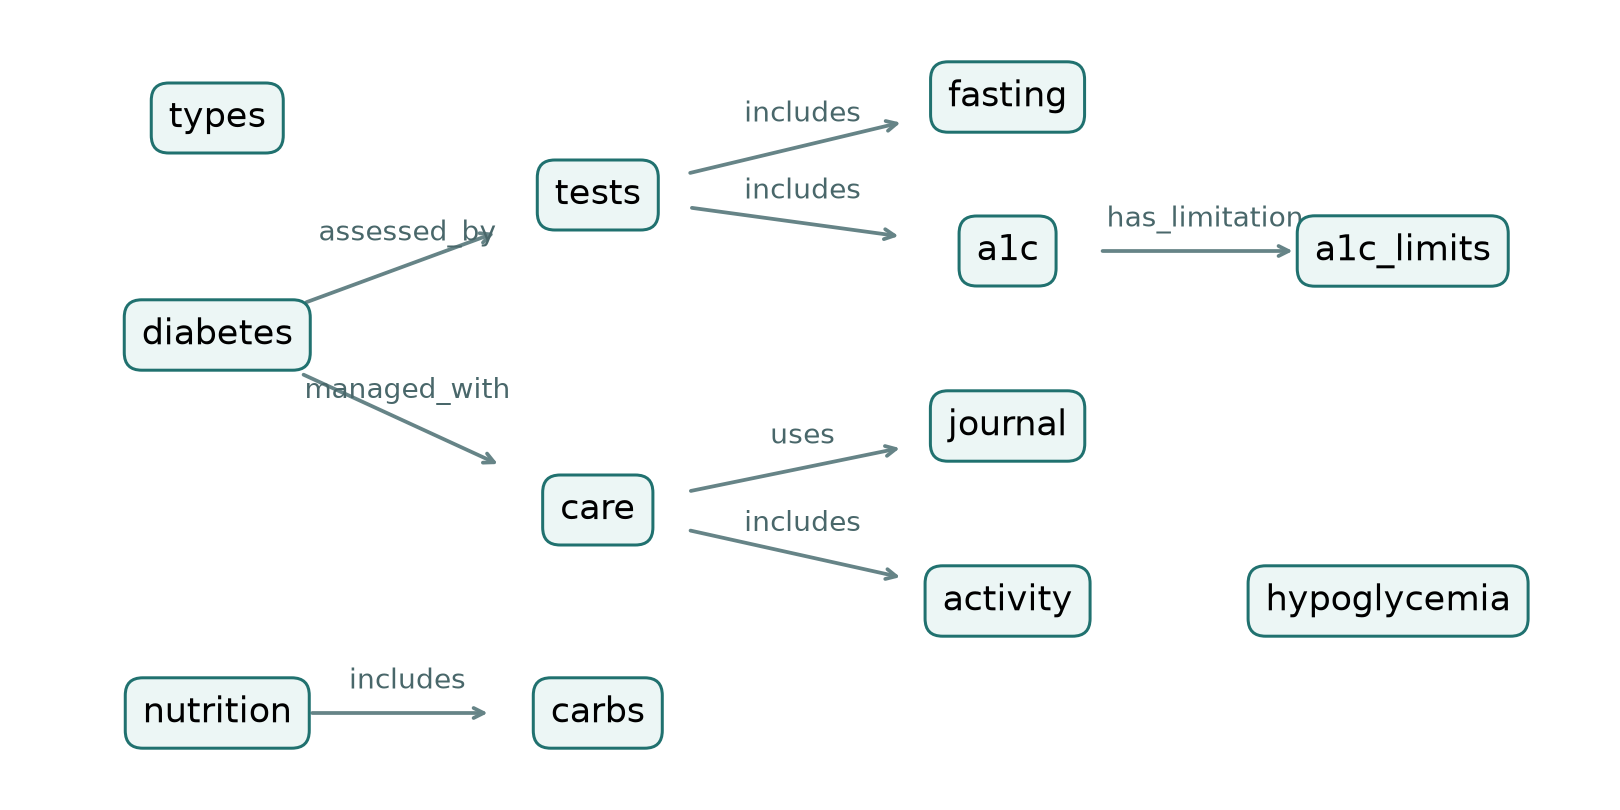
\includegraphics[width=\textwidth]{images/knowledge_graph.png}
\caption{Đồ thị 12 khái niệm và các quan hệ được biên soạn trong project. Các ghi chú D01--D12 được gắn cạnh bằng chứng trong JSON.}
\end{figure}

Graph được lưu bằng JSON và nạp trực tiếp khi ứng dụng khởi động. File \path{concept_graph.cypher} xuất nút/cạnh khái niệm để tham khảo nếu muốn tiếp tục với Neo4j; bản local không yêu cầu cài Neo4j và chưa được đánh giá trên một Neo4j server. Không gọi cách mở rộng nhỏ này là triển khai đầy đủ các phương pháp GraphRAG quy mô lớn.

\section{Truy xuất và kết xuất câu trả lời}
Văn bản được chuẩn hóa chữ thường và bỏ dấu, sau đó vector hóa TF-IDF với unigram/bigram. Corpus đầu vào cho từng ghi chú gồm tiêu đề, từ khóa và nội dung. Điểm lexical là cosine similarity giữa query và mỗi ghi chú. Alias khớp theo ranh giới từ giúp xác định các concept được nhắc trực tiếp.

Khi bật đồ thị, hệ thống mở rộng một bước theo cạnh có hướng. Ghi chú thuộc các concept trực tiếp hoặc mở rộng được cộng 0,12 vào điểm lexical. Để tránh suy ra bằng chứng chỉ vì ở gần trong graph, ứng viên phải có cosine ít nhất 0,10 nếu không khớp concept trực tiếp. Ngoài ra, ứng viên cần khớp alias hoặc có ít nhất hai token query ở tiêu đề/từ khóa sau khi bỏ một số từ chức năng.

\begin{equation}
\operatorname{score}(d,q)=\cos\bigl(v_d,v_q\bigr)+0,12\,\mathbb{1}\{C_d\cap C_q^{+}\ne\varnothing\}.
\end{equation}
Các điều kiện trên là heuristic được định nghĩa trong source; chưa có tập phát triển độc lập để chứng minh ngưỡng tối ưu. Chúng ngăn một số kết quả do trùng từ thông thường nhưng cũng có thể làm bỏ sót cách diễn đạt mới.

Tối đa ba ghi chú được trả về theo điểm, nếu bằng điểm thì theo ID. Không có ứng viên đạt thì trả insufficient\_evidence. Câu trả lời nối trực tiếp nội dung ghi chú cùng ID, còn giao diện hiển thị URL tương ứng. Đây là RAG theo kiểu truy xuất và kết xuất trích đoạn theo mẫu, không dùng LLM hoặc embedding model. Council kiểm tra tính hợp lệ của ID nhưng không chứng minh độ liên quan ngữ nghĩa của từng đoạn.

\section{Thiết kế đánh giá truy xuất}
Bộ đánh giá có 24 câu do tác giả soạn, mỗi ghi chú hai câu và một ID đích. Hit@1 kiểm tra kết quả đầu; Hit@3 kiểm tra ID xuất hiện trong ba kết quả; MRR lấy trung bình nghịch đảo thứ hạng, bằng 0 nếu không tìm thấy. Cùng bộ câu được chạy có và không có bonus đồ thị để xem đóng góp của thành phần này.

Bộ câu nhỏ và dùng từ vựng gần KB, nên không đại diện câu hỏi người bệnh ngoài thực tế. Các bài kiểm tra đã giúp phát hiện lỗi trong quá trình phát triển; vì vậy kết quả cuối là bằng chứng hồi quy và chức năng, không phải một test truy xuất độc lập chưa từng được xem. Báo cáo không dùng điểm cao để tuyên bố khả năng hiểu hội thoại y tế tổng quát.

\section{MDP nhắc ghi nhật ký}
Nhánh RL minh họa cách tác tử cải thiện chính sách qua phản hồi. Mục tiêu là cân bằng việc có bản ghi với chi phí và cảm giác mệt do thông báo. Mọi hệ số phản ứng/phần thưởng dưới đây do tác giả đặt để tạo môi trường học, không được ước lượng từ bệnh nhân hoặc thử nghiệm y khoa.

Trạng thái có dạng $s=2g+f$, trong đó $g\in\{0,1,2,3\}$ là số ngày chưa ghi, được chặn tại 3, và $f\in\{0,1\}$ là trạng thái mệt vì thông báo. Có 8 trạng thái và 3 hành động: $a=0$ không nhắc, $a=1$ nhắc ghi nhật ký, $a=2$ gửi gợi ý ghi chép ngắn. Reminder chỉ quyết định hành động trong tập này.

Xác suất ghi nhận ở bước tiếp theo được mô phỏng:
\begin{equation}
P(L=1\mid g,f,a)=\operatorname{clip}\bigl(0,40-0,07g-0,08f+b_a;\ 0,05;\ 0,95\bigr),
\end{equation}
với $b_a\in\{0;0,35;0,22\}$. Nếu có bản ghi, $g'=0$; nếu không, $g'=\min(3,g+1)$. Xác suất mệt ở ngày tiếp theo là 0,15; 0,70 hoặc 0,40 theo hành động tương ứng. Reward:
\begin{equation}
r=L-c_a-0,10g'-0,12f\mathbb{1}\{a>0\}, \qquad c_a\in\{0;0,22;0,10\}.
\end{equation}
Một policy có reward cao hơn chỉ phù hợp hơn với utility của simulator này. Reward không có đơn vị đường huyết và không đo mức cải thiện sức khỏe.

\section{Huấn luyện Q-learning}
Theo quy tắc Q-learning \cite{watkins}, tác tử cập nhật:
\begin{equation}
Q(s,a)\leftarrow Q(s,a)+\alpha\left[r+\gamma\max_{a'}Q(s',a')-Q(s,a)\right].
\end{equation}
Project dùng $\alpha=0,08$, $\gamma=0,92$, $\epsilon$-greedy với $\epsilon_e=\max(0,03;0,8\cdot0,997^e)$. Mỗi seed train có 1.800 episode, mỗi rollout 28 ngày. Đây là bài toán continuing: mốc 28 ngày chỉ là cửa sổ lấy mẫu, không phải trạng thái bệnh kết thúc, nên bước cuối vẫn bootstrap từ Q của trạng thái kế.

Năm seed train là 42--46. Mỗi policy được đánh giá greedy bằng 200 seed 10000--10199, tách khỏi seed train. Các policy đối chứng gồm không bao giờ nhắc, luôn nhắc và luật chỉ nhắc khi gap từ 2 và chưa mệt. Các lượt eval dùng cùng seed giữa policy để giảm nhiễu so sánh.

Q-table của seed 42 được dùng trong demo theo quy định trước. Project không chọn seed đạt điểm cao nhất. Độ lệch chuẩn trong bảng tổng hợp là độ biến thiên giữa năm reward trung bình của các seed train, không phải khoảng tin cậy lâm sàng.

\section{Kết hợp luật với chính sách}
Intake có thể dừng toàn bộ request trước khi Reminder được gọi. Council bác các proposal medication; action space của Reminder cũng không có hành động dùng thuốc. Khi gap/fatigue sai mã, Reminder trả needs\_input thay vì tự cắt giá trị vào miền hợp lệ. Như vậy, kết quả học được không được dùng để vượt qua giới hạn đầu vào và phạm vi hệ thống.

Project chưa học policy từ dữ liệu hành vi thật, chưa kiểm tra offline policy evaluation, chưa mô hình hóa sở thích cá nhân hoặc ràng buộc dài hạn. Việc mở rộng chỉ có ý nghĩa khi có dữ liệu và thiết kế nghiên cứu phù hợp; không suy rộng từ bảng Q nhỏ sang chính sách chăm sóc thực tế.

\chapter{Cài đặt và giải thích mã nguồn}
\section{Tổ chức mã nguồn}
Các module trong \path{diabetes_agent/} được dùng chung bởi notebook và giao diện. \path{data.py} đọc dữ liệu; \path{models.py} huấn luyện và suy luận; \path{knowledge.py} truy xuất tri thức; \path{rl.py} cài đặt môi trường và Q-learning; \path{system.py} quản lý thông điệp và điều phối. \path{app.py} nhận đầu vào, gọi hệ thống và hiển thị kết quả.

Các đoạn mã trong phần này được trích từ source của Project01. Tên tệp và số dòng được ghi phía trên mỗi đoạn; số dòng bên trái giữ theo tệp gốc.

\section{Đọc dữ liệu và kiểm tra chia tập}
\reportcode{data_check}{Đọc CSV và kiểm tra tính toàn vẹn dữ liệu.}

Hàm \texttt{load\_data} đọc checksum từ \path{provenance.json}, tính SHA256 của CSV rồi so sánh trước khi nạp bảng. Hai phép kiểm tra sau đó xác nhận nhãn thuộc tập $\{0,1\}$ và 21 cột đầu vào không có giá trị thiếu.

Biến \texttt{groups} chứa tập mã nhóm của train, validation và test. Phép giao giữa các tập được kiểm tra để phát hiện nhóm xuất hiện ở nhiều split. Phần cuối tính lại fingerprint từ chính 21 đặc trưng; nếu một fingerprint thuộc nhiều split, biểu thức \texttt{nunique().max()} lớn hơn 1 và chương trình dừng. Kết quả trả về là DataFrame đã qua các kiểm tra này.

\section{Mạng MLP và chuẩn hóa đầu vào}
\reportcode{architecture}{Kiến trúc MLP sử dụng trong huấn luyện và suy luận.}

\texttt{nn.Linear(21,64)} ánh xạ 21 chỉ báo vào lớp ẩn thứ nhất. ReLU tạo phi tuyến; dropout 0,15 được áp dụng khi huấn luyện. Lớp ẩn thứ hai có 32 nút, sau đó lớp cuối trả một logit. Sigmoid được áp dụng khi suy luận để tạo score trong khoảng $[0,1]$.

\reportcode{train_setup}{Chuẩn hóa dữ liệu và khởi tạo bộ tối ưu.}

Scaler chỉ được fit bằng \texttt{train[FEATURES]}; cùng scaler đó biến đổi train và validation. Tensor đặc trưng có 21 cột, còn \texttt{reshape(-1,1)} đưa nhãn về cùng dạng với đầu ra mạng. Loss là \texttt{BCEWithLogitsLoss}; Adam sử dụng learning rate 0,001 và weight decay $10^{-4}$. Biến \texttt{best\_loss} lưu loss validation thấp nhất, còn \texttt{stale} đếm số epoch liên tiếp không cải thiện.

\section{Vòng huấn luyện và lưu checkpoint}
\reportcode{train_loop}{Huấn luyện minibatch và chọn checkpoint theo validation.}

Ở đầu mỗi epoch, \texttt{net.train()} bật chế độ huấn luyện và \texttt{randperm} xáo trộn thứ tự mẫu. Các chỉ số được chia thành minibatch 256 phần tử. Trong mỗi batch, gradient cũ được xóa, mạng tính logit, loss lan truyền ngược rồi Adam cập nhật tham số. Tổng loss được nhân với số mẫu của batch để tính trung bình theo mẫu.

Sau vòng minibatch, \texttt{net.eval()} tắt dropout; \texttt{torch.no\_grad()} tính loss validation mà không lưu đồ thị gradient. Khi loss giảm hơn $10^{-5}$, chương trình sao chép \texttt{state\_dict} và đặt lại \texttt{stale}. Nếu 10 epoch liên tiếp không đạt mức cải thiện này, vòng lặp kết thúc. Mạng cuối cùng nạp lại checkpoint có loss validation thấp nhất; ở lần chạy báo cáo, checkpoint thuộc epoch 21.

\section{Chọn ngưỡng và mô hình mặc định}
\reportcode{threshold}{Chọn ngưỡng phân loại bằng F1 validation.}

Hàm thử 151 ngưỡng từ 0,05 đến 0,80. Với từng ngưỡng $t$, dự đoán nhị phân là \texttt{p >= t}; hàm trả ngưỡng có F1 cao nhất. Thứ tự tăng dần của danh sách ngưỡng làm cho trường hợp bằng điểm chọn ngưỡng nhỏ hơn.

\reportcode{model_selection}{Tổng hợp validation và lưu quyết định chọn mô hình.}

Mỗi mô hình trả score trên validation, sau đó tính các chỉ số tại ngưỡng riêng. Dummy được giữ trong bảng đối chứng nhưng bị loại khỏi nhóm ứng viên mặc định. Các mô hình còn lại được sắp giảm dần theo Average Precision; tên mô hình đứng đầu và các ngưỡng được ghi vào manifest. Tập test được đánh giá ở bước sau bằng các quyết định đã lưu này.

\section{Suy luận từ mô hình đã lưu}
\reportcode{inference}{Hàm dự đoán của lớp RiskModel.}

Giá trị \texttt{default} được thay bằng tên trong manifest. Câu lệnh \texttt{[FEATURES]} cố định thứ tự 21 cột, tránh thay đổi vị trí đặc trưng khi hồ sơ JSON có thứ tự khóa khác. Nhánh MLP áp dụng scaler, tạo tensor, chạy mạng ở chế độ suy luận rồi lấy sigmoid; các mô hình sklearn trả cột xác suất của lớp 1 qua \texttt{predict\_proba}.

Ngưỡng được đọc theo đúng model ID. Hàm trả score, threshold và biến \texttt{positive} từ phép so sánh giữa hai giá trị. Các trường này được dùng trực tiếp để dựng vòng điểm và nhãn trên dashboard.

\section{Truy xuất tri thức}
\reportcode{retrieval}{TF-IDF kết hợp mở rộng khái niệm một bước.}

Hàm chuẩn hóa query rồi tính cosine similarity với ma trận TF-IDF của 12 ghi chú. Biến \texttt{concepts} chứa những khái niệm có alias khớp query theo ranh giới từ. Khi bật graph, các đích của cạnh đi ra từ tập này được thêm vào \texttt{expanded}; vòng mở rộng chỉ chạy trên tập ban đầu nên dừng ở một bước.

Với mỗi ghi chú, \texttt{matched} xác định các khái niệm giao với tập mở rộng. Bonus bằng 0,12 nếu có liên kết phù hợp. Bộ lọc yêu cầu khớp concept trực tiếp hoặc có ít nhất hai token trùng ở tiêu đề/từ khóa; cosine dưới 0,10 cũng bị loại nếu không khớp trực tiếp. Kết quả được sắp theo score giảm dần, dùng ID để xử lý hòa điểm và lấy tối đa $k=3$ ghi chú.

\section{Cập nhật bảng Q}
\reportcode{q_learning}{Huấn luyện Q-learning cho tác tử nhắc nhật ký.}

Mảng \texttt{q} có kích thước $8\times3$, tương ứng tám trạng thái và ba hành động. Bộ sinh ngẫu nhiên được tạo từ seed truyền vào. Ở mỗi episode, tác tử chọn hành động ngẫu nhiên với xác suất epsilon; các lượt còn lại chọn \texttt{argmax} của hàng Q ứng với trạng thái hiện tại.

Hàm \texttt{transition} trả trạng thái kế tiếp và reward. Dòng cập nhật sử dụng learning rate 0,08, hệ số chiết khấu 0,92 và giá trị Q lớn nhất tại trạng thái kế tiếp. Sau 28 ngày, reward trung bình của episode được đưa vào history. Hàm trả cả bảng Q và DataFrame lịch sử; thí nghiệm gọi hàm với năm seed 42--46.

\section{Giao tiếp và kiểm tra kết quả tác tử}
\reportcode{message_bus}{Gửi yêu cầu và ghi thông điệp phản hồi qua MessageBus.}

MessageBus ghi một REQUEST trước khi gọi handler của bên nhận. Thời gian thực thi được đo bằng \texttt{perf\_counter}. Kết quả thành công được ghi dưới dạng INFORM; exception được chuyển thành dữ liệu có trạng thái failure và thông điệp FAILURE. Lỗi tại một handler vẫn có mặt trong trace để Coordinator và Council xử lý.

\reportcode{council}{Các điều kiện kiểm tra của Council.}

Council duyệt từng proposal, tích lũy lý do bác trong \texttt{reasons}. Các điều kiện gồm đề xuất loại medication, lỗi failure, kết quả tri thức thiếu bằng chứng hoặc chứa ID ngoài kho và score ngoài khoảng $[0,1]$. Hàm chỉ trả approved khi danh sách lý do rỗng; các trường hợp còn lại trả rejected kèm lý do.

\section{Điều phối một lượt xử lý}
\reportcode{coordination}{Nhánh tiếp nhận, gọi chuyên gia và tổng hợp của Coordinator.}

Intake được gọi trước. Trạng thái khác completed tạo kết quả kết thúc với danh sách proposal rỗng. Nếu tiếp nhận thành công, tác vụ consult gọi cả Risk, Knowledge và Reminder; các tác vụ riêng chỉ gọi chuyên gia tương ứng. Tất cả proposal được chuyển tới Council trước khi Advisor tổng hợp.

Khi Council bác kết quả, trạng thái chung là rejected. Khi được duyệt, Advisor trả văn bản tổng hợp; trạng thái chung vẫn là needs\_input nếu một chuyên gia yêu cầu bổ sung dữ liệu, hoặc insufficient\_evidence nếu nhánh tri thức thiếu căn cứ. Việc duyệt cấu trúc proposal được tách khỏi tình trạng hoàn thành của nhiệm vụ.

\section{Liên kết mã nguồn với giao diện}
\reportcode{ui_presets}{Callback của ba kịch bản chạy nhanh.}

Callback đặt tác vụ, câu hỏi và nguồn hồ sơ vào \texttt{st.session\_state}, sau đó gọi \texttt{system.run}. Kết quả được lưu vào khóa \texttt{result}. Các kịch bản dùng cùng tham số nhắc việc và model đang được chọn trên giao diện, nên thao tác chạy nhanh đi qua cùng luồng xử lý với nút Bắt đầu phân tích.

\reportcode{ui_flow}{Dựng trạng thái hiển thị của bảy vai trò tác tử.}

Hàm lấy các phản hồi trong trace theo tên tác tử và ánh xạ completed/approved sang trạng thái done. Các phản hồi khác được hiển thị attention; tác tử chưa có phản hồi giữ trạng thái idle. Coordinator dùng trạng thái tổng của phiên. Màu của các thẻ trên dashboard phản ánh vết xử lý đã ghi.

\section{Notebook và các tệp kết quả}
\begin{table}[H]\centering\small
\caption{Nội dung và đầu ra của bốn notebook.}
\begin{tabularx}{\textwidth}{@{}p{1cm}p{4.2cm}Y@{}}\toprule
Số & Nội dung & Đầu ra chính \\\midrule
01 & Dữ liệu và MLP & Bộ chia tập, checkpoint, scaler, bảng validation/test và prediction từng dòng. \\
02 & Tri thức và đồ thị & Danh mục ghi chú, ví dụ truy xuất và đánh giá 24 câu hỏi. \\
03 & Q-learning & Bảng Q seed 42, lịch sử năm seed và so sánh policy. \\
04 & Tích hợp hệ đa tác tử & Kết quả hội chẩn, trace, nhánh dữ liệu thiếu/cảnh báo và đánh giá hệ thống. \\\bottomrule
\end{tabularx}
\end{table}

Bốn notebook có tổng cộng 26 code cell đã thực thi. Mô hình và các bảng số liệu được lưu trong \path{artifacts/}; nhật ký demo tùy chọn được lưu riêng tại \path{artifacts/demo_audit.sqlite3}.

\chapter{Thực nghiệm và phân tích kết quả}
\section{Điều kiện thực nghiệm}
Các thực nghiệm chạy trên CPU với Python 3.11.9, PyTorch 2.15.0+cpu, scikit-learn 1.9.1, pandas 2.3.3 và Streamlit 1.66.1. Phiên bản trực tiếp được ghi trong requirements, còn môi trường kiểm tra đầy đủ nằm ở \texttt{artifacts/environment.txt}. Môi trường cài mới trên máy khác chưa được kiểm chứng; việc bàn giao xác nhận source và artifact chạy trong môi trường nêu trên.

Dữ liệu supervised dùng một split/seed cố định. RL chạy năm seed train và các seed eval tách biệt. Đánh giá phần mềm và truy xuất sử dụng kịch bản do tác giả xây. Mỗi loại bằng chứng trả lời một câu hỏi khác nhau: test supervised đo phân loại nội bộ, simulator đo utility giả định, bộ tình huống đo tuân thủ hợp đồng. Không gộp các điểm này thành một tỷ lệ chính xác chung của hệ thống y tế.

\section{Kết quả validation và lựa chọn mặc định}
\begin{table}[H]\centering\small
\caption{Chỉ số trên validation; ngưỡng được chọn bằng F1 validation.}
\begin{tabular}{@{}lrrrrrr@{}}\toprule
Model & AUC & AP & F1 & Precision & Recall & Brier \\\midrule
dummy & 0.5000 & 0.1314 & 0.2322 & 0.1314 & 1.0000 & 0.1142 \\
logistic & 0.8127 & 0.3482 & 0.4350 & 0.3397 & 0.6047 & 0.0986 \\
random\_forest & 0.8104 & 0.3713 & 0.4387 & 0.3383 & 0.6237 & 0.0967 \\
mlp & 0.8170 & 0.3706 & 0.4414 & 0.3285 & 0.6723 & 0.0960 \\
\bottomrule\end{tabular}
\end{table}
Random Forest có Average Precision validation khoảng 0,3713, nhỉnh hơn MLP khoảng 0,3706. Theo quy tắc đã đặt, Random Forest được chọn làm model mặc định. MLP có ROC AUC validation cao hơn, nhưng tiêu chí chọn đã khóa là AP nên không đổi sang AUC sau khi thấy bảng kết quả.

Chênh lệch AP giữa hai model rất nhỏ và chưa có phân tích độ bất định để kết luận model nào tốt hơn ổn định. Lựa chọn mặc định chỉ là kết quả áp dụng quy tắc trong lần chia tập này. Giao diện vẫn cho chọn MLP để trình diễn nhánh học sâu và so sánh với các baseline.

\section{Kết quả trên test đã khóa}
\begin{table}[H]\centering\small
\caption{Chỉ số trên test; ngưỡng được chọn bằng F1 validation.}
\begin{tabular}{@{}lrrrrrr@{}}\toprule
Model & AUC & AP & F1 & Precision & Recall & Brier \\\midrule
dummy & 0.5000 & 0.1373 & 0.2415 & 0.1373 & 1.0000 & 0.1185 \\
logistic & 0.8118 & 0.3820 & 0.4367 & 0.3499 & 0.5806 & 0.1003 \\
random\_forest & 0.8096 & 0.3906 & 0.4534 & 0.3564 & 0.6230 & 0.0993 \\
mlp & 0.8168 & 0.3916 & 0.4431 & 0.3358 & 0.6512 & 0.0987 \\
\bottomrule\end{tabular}
\end{table}
\begin{table}[H]\centering\small
\caption{Ngưỡng đã khóa và số lượng dự đoán trên test.}
\begin{tabular}{@{}lrrrrrr@{}}\toprule
Model & Ngưỡng & TN & FP & FN & TP & Specificity \\\midrule
dummy & 0.050 & 0 & 3116 & 0 & 496 & 0.0000 \\
logistic & 0.215 & 2581 & 535 & 208 & 288 & 0.8283 \\
random\_forest & 0.230 & 2558 & 558 & 187 & 309 & 0.8209 \\
mlp & 0.205 & 2477 & 639 & 173 & 323 & 0.7949 \\
\bottomrule\end{tabular}
\end{table}

\noindent\textbf{Quan sát.} MLP đạt ROC AUC khoảng 0,8168 và AP khoảng 0,3916; Random Forest đạt AUC khoảng 0,8096 và AP khoảng 0,3906. Logistic Regression đạt AUC khoảng 0,8118. Các model học được đều có AP cao hơn Dummy khoảng 0,1373, là tỷ lệ lớp dương trong test.

\noindent\textbf{Diễn giải.} MLP nhỉnh hơn về AUC/AP trên test nhưng không làm thay đổi quyết định mặc định đã khóa từ validation. Các chênh lệch này là mô tả trên cùng split, chưa đủ để khẳng định ưu thế tổng quát. Mô hình bảng đơn giản hơn vẫn là đối chứng cần thiết cho một mạng hai lớp ẩn.

\noindent\textbf{Đánh đổi tại ngưỡng.} MLP phát hiện 323/496 mẫu lớp 1, còn bỏ sót 173 mẫu và tạo 639 dương tính giả. Random Forest phát hiện 309 mẫu, bỏ sót 187 và tạo 558 dương tính giả. Khi tăng recall, precision có thể giảm; việc chọn F1 validation không đồng nghĩa chọn ngưỡng phù hợp cho quyết định lâm sàng.

\begin{figure}[H]\centering
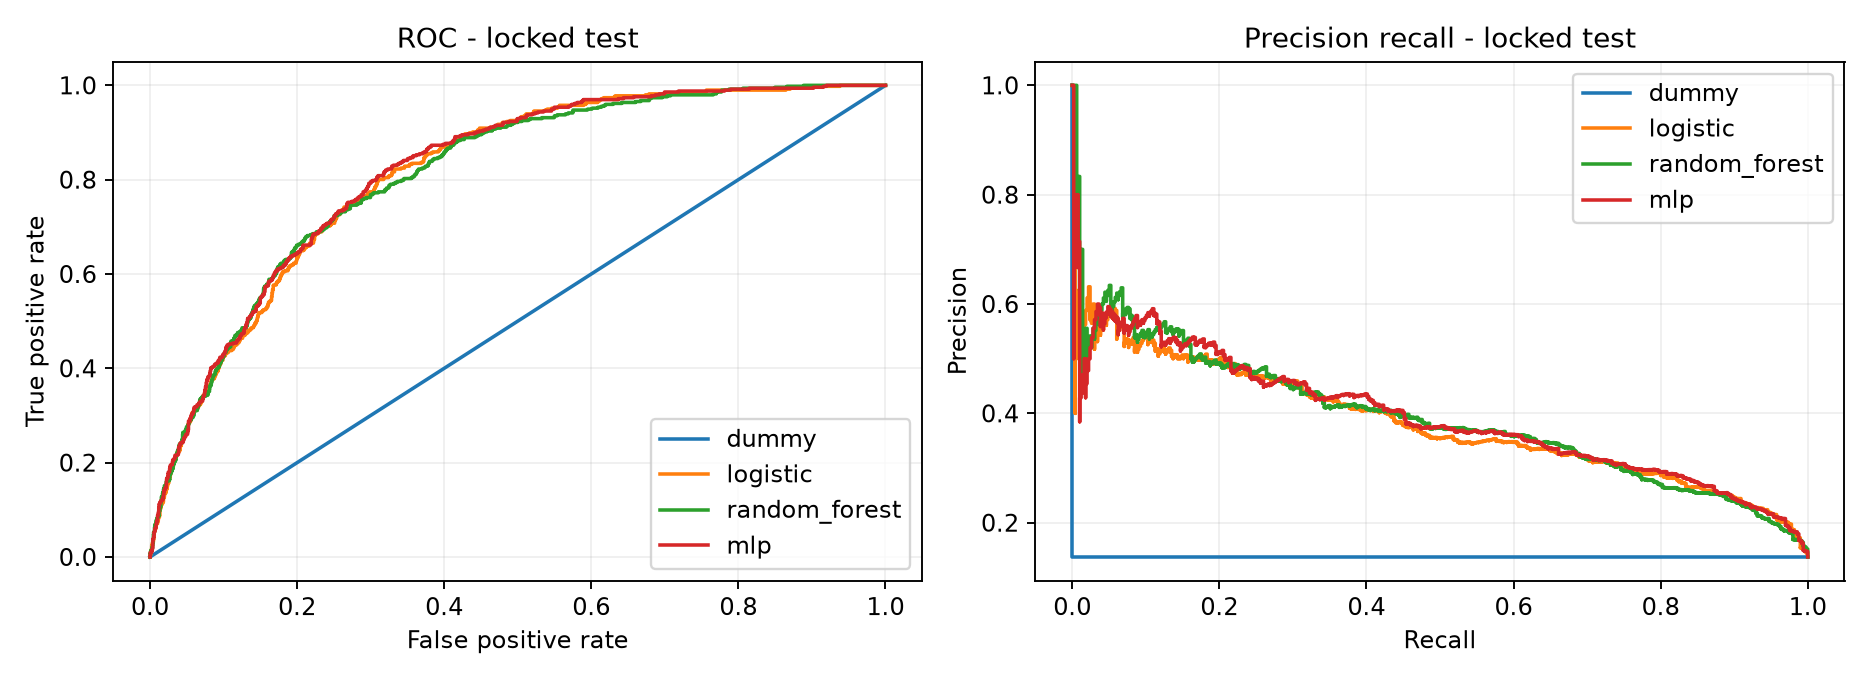
\includegraphics[width=\textwidth]{images/classification.png}
\caption{ROC và Precision--Recall trên test. Mọi quyết định về model/ngưỡng được thực hiện bằng validation trước đó.}
\end{figure}

Dummy được chọn ngưỡng nhỏ hơn điểm tiên nghiệm nên dự đoán tất cả là lớp 1, dẫn tới recall 1 và specificity 0. Điều này minh họa vì sao một chỉ số riêng lẻ có thể gây hiểu nhầm. Cần đọc đồng thời precision, recall và số lượng FP/FN.

\section{Quá trình học của MLP}
\begin{figure}[H]\centering
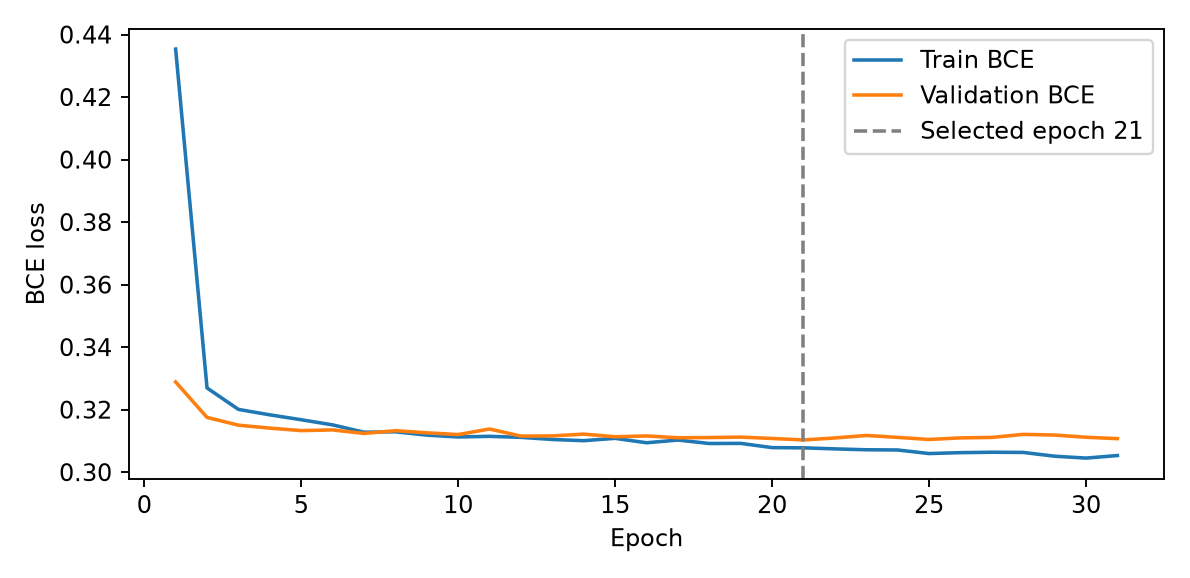
\includegraphics[width=0.92\textwidth]{images/training.png}
\caption{Loss train và validation, đường dọc thể hiện epoch được chọn để lưu checkpoint.}
\end{figure}

Checkpoint MLP được chọn tại epoch 21 theo BCE validation. Train tiếp tục cho tới khi đủ số epoch không cải thiện rồi nạp lại checkpoint tốt nhất. Train loss và validation loss không nhất thiết cùng giảm ở các epoch cuối; đó là lý do giữ checkpoint dựa trên tập không tham gia cập nhật gradient.

Brier test của MLP khoảng 0,0987, thấp hơn Dummy khoảng 0,1185. Đây là dấu hiệu mô hình cung cấp score hữu ích hơn tiên nghiệm trong điều kiện test nội bộ. Chưa có đường calibration theo nhóm, khoảng tin cậy hoặc đánh giá dịch chuyển phân bố nên không thể chuyển score đó thành nguy cơ cá nhân ở Việt Nam.

\section{Truy xuất tri thức và vai trò đồ thị}
\begin{table}[H]\centering\small
\caption{Đánh giá truy xuất trên 24 câu hỏi của bộ thực nghiệm.}
\begin{tabular}{@{}lrrr@{}}\toprule
Cấu hình & Hit@1 & Hit@3 & MRR \\\midrule
TF-IDF & 1.0000 & 1.0000 & 1.0000 \\
TF-IDF + graph & 1.0000 & 1.0000 & 1.0000 \\
\bottomrule\end{tabular}
\end{table}

Cả hai cấu hình đều tìm đúng ID đầu tiên ở toàn bộ 24 câu trong phiên bản cuối. Vì vậy, bộ câu hiện tại không cho thấy lợi ích đo được của bonus đồ thị về Hit@1, Hit@3 hoặc MRR. Đồ thị vẫn có chức năng biểu diễn liên kết và mở rộng concept trong implementation, nhưng chưa có bằng chứng nó làm tăng chất lượng trên tập kiểm tra này.

Điểm tuyệt đối cần được đọc cùng giới hạn thiết kế: chỉ 12 ghi chú, câu hỏi do chính tác giả viết và dùng lại để kiểm tra trong phát triển. Không có bộ paraphrase độc lập hoặc đánh giá từ người dùng. Một bước tiếp theo có giá trị là thu thập câu hỏi ngoài từ vựng KB, nhiều chủ đề và trường hợp cần từ chối, rồi khóa bộ test riêng.

\section{Kết quả Q-learning và đối chứng}
\begin{table}[H]\centering\small
\caption{Reward mỗi ngày trong simulator; std giữa năm giá trị trung bình theo seed train.}
\begin{tabular}{@{}lrr@{}}\toprule
Policy & Reward trung bình & Độ lệch chuẩn \\\midrule
fixed & 0.2868 & 0.0000 \\
never & 0.0876 & 0.0000 \\
q\_learning & 0.2703 & 0.0153 \\
rule & 0.2006 & 0.0000 \\
\bottomrule\end{tabular}
\end{table}
\begin{figure}[H]\centering
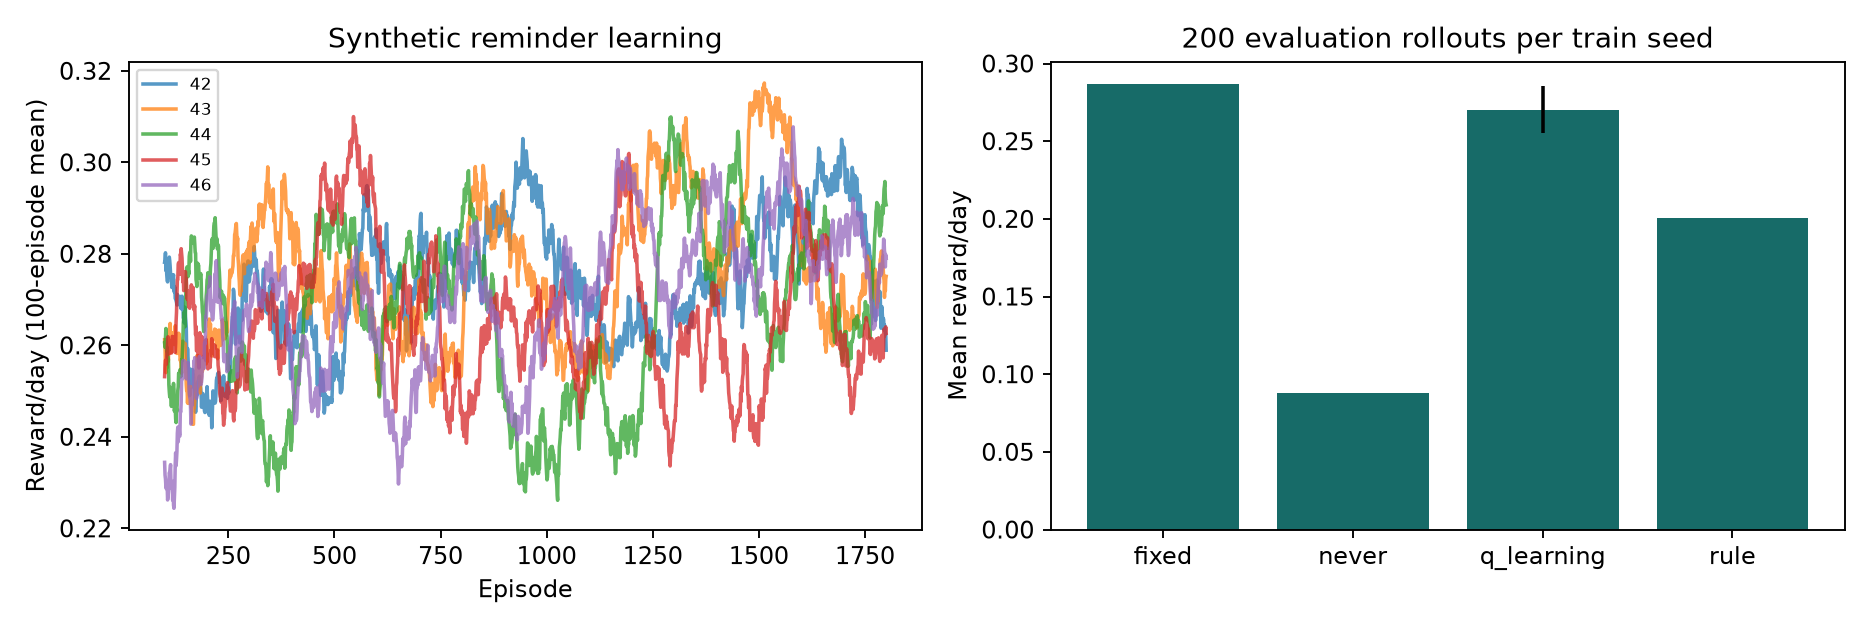
\includegraphics[width=\textwidth]{images/rl.png}
\caption{Đường học năm seed và reward đánh giá trong môi trường nhắc việc giả lập.}
\end{figure}

\noindent\textbf{Quan sát.} Q-learning có reward trung bình khoảng 0,2703 mỗi ngày, cao hơn never khoảng 0,0876 và rule khoảng 0,2006, nhưng thấp hơn fixed khoảng 0,2868. Độ lệch chuẩn giữa năm seed train của Q-learning khoảng 0,0153.

\noindent\textbf{Diễn giải.} Trong simulator này, lợi ích ghi nhận do hành động nhắc thường bù được chi phí nên policy luôn nhắc là đối chứng mạnh. Q-learning hữu hạn với learning rate cố định và năm seed chưa vượt đối chứng đó. Kết quả không được sửa bằng cách đổi reward sau khi xem điểm; báo cáo giữ nguyên cả trường hợp RL không tốt nhất.

\noindent\textbf{Giới hạn của phép đo.} Fixed/never/rule có std giữa seed train bằng 0 vì cùng policy được đánh giá lại với cùng 200 seed eval, không phải vì mọi rollout có reward giống nhau. Các dòng lặp của đối chứng không tạo thêm mẫu độc lập. Q-table seed 42 được nạp trong demo theo quy ước trước, không chọn theo reward eval.

\section{Kiểm tra tích hợp và lỗi được inject}
\begin{table}[H]\centering\small
\caption{Các kịch bản chức năng được chạy ở phiên bản bàn giao.}
\begin{tabular}{@{}llcr@{}}\toprule
Kịch bản & Trạng thái mong đợi & Đạt & Thông điệp \\\midrule
risk\_complete & completed & Có & 8 \\
risk\_mlp & completed & Có & 8 \\
risk\_missing & needs\_input & Có & 8 \\
risk\_invalid & needs\_input & Có & 8 \\
risk\_nan & needs\_input & Có & 8 \\
knowledge\_a1c & completed & Có & 8 \\
knowledge\_food & completed & Có & 8 \\
knowledge\_activity & completed & Có & 8 \\
knowledge\_unknown & insufficient\_evidence & Có & 8 \\
knowledge\_blank & insufficient\_evidence & Có & 8 \\
urgent\_text & urgent & Có & 2 \\
urgent\_seizure & urgent & Có & 2 \\
urgent\_glucose & urgent & Có & 2 \\
invalid\_unit\_value & needs\_input & Có & 2 \\
medication & out\_of\_scope & Có & 2 \\
reminder & completed & Có & 8 \\
invalid\_reminder & needs\_input & Có & 8 \\
consult & completed & Có & 12 \\
consult\_missing & needs\_input & Có & 12 \\
consult\_unknown & insufficient\_evidence & Có & 12 \\
\bottomrule\end{tabular}
\end{table}
Toàn bộ 20 kịch bản đạt trạng thái mong đợi ở phiên bản bàn giao. Kịch bản phủ luồng dự đoán, dữ liệu thiếu/sai mã, query có/không có bằng chứng, số đo bổ sung không hợp lệ, nhánh khẩn cấp, phạm vi thuốc và reminder. Đây là tỷ lệ đạt bộ yêu cầu phần mềm hữu hạn, không phải tỷ lệ tư vấn đúng trong mọi tình huống.

Sáu proposal lỗi được inject riêng gồm thuốc, tri thức không nguồn, ID giả, score vượt khoảng, score NaN và lỗi handler. Council bác cả sáu. Ở cấu hình bỏ Council, các proposal được đánh dấu unreviewed; không gọi đó là đã qua kiểm tra hoặc đã gây hại. Phép ablation xác nhận chức năng veto đối với lỗi được dựng sẵn, chưa chứng minh MAS tốt hơn một pipeline đơn tác tử dùng cùng luật và công cụ.

\section{Kiểm thử tự động và notebook}
Bộ pytest có 28 trường hợp và đều đạt. Các nhóm kiểm tra gồm checksum/fingerprint, mã khảo sát không hợp lệ, score nạp lại khớp prediction, ưu tiên urgent trước Risk, nguồn cảnh báo glucose, truy xuất không dấu và từ chối ngoài chủ đề, Council veto, cô lập exception trong bus, tính tái lập Q, miền trạng thái, ghi/đọc audit và thao tác UI bằng Streamlit AppTest.

Bốn notebook có lần lượt 7, 6, 5 và 8 code cell, tổng cộng 26 cell. Tất cả có execution count và không có error output. Log lưu tên file, số cell và thời gian thực thi. Việc kiểm tra trực tiếp bằng trình duyệt còn được dùng để quan sát màu chữ, bố cục và ảnh minh chứng, bổ sung cho kiểm thử cấu trúc bằng AppTest.


\chapter{Giao diện và kết quả chạy demo}
\section{Dashboard tổng quan}
Giao diện Streamlit tổ chức thành bốn tab: Hội chẩn demo, Tri thức và đồ thị, Thực nghiệm, Hướng dẫn. Phần đầu hiển thị tên hệ thống, quy mô dữ liệu, số tác tử và số ghi chú. Các nút chạy nhanh nạp đồng thời câu hỏi, hồ sơ và dữ liệu nhật ký của từng tình huống.

Trong tab hội chẩn, vùng nhập liệu gồm lựa chọn tác vụ, mô hình, câu hỏi và hồ sơ 21 chỉ báo. Hồ sơ mẫu lấy từ tập train; chế độ Nhập JSON cho phép thay toàn bộ vector đầu vào. Trạng thái của bảy tác tử được cập nhật từ thông điệp phát sinh khi chạy hệ thống.
\begin{figure}[H]\centering
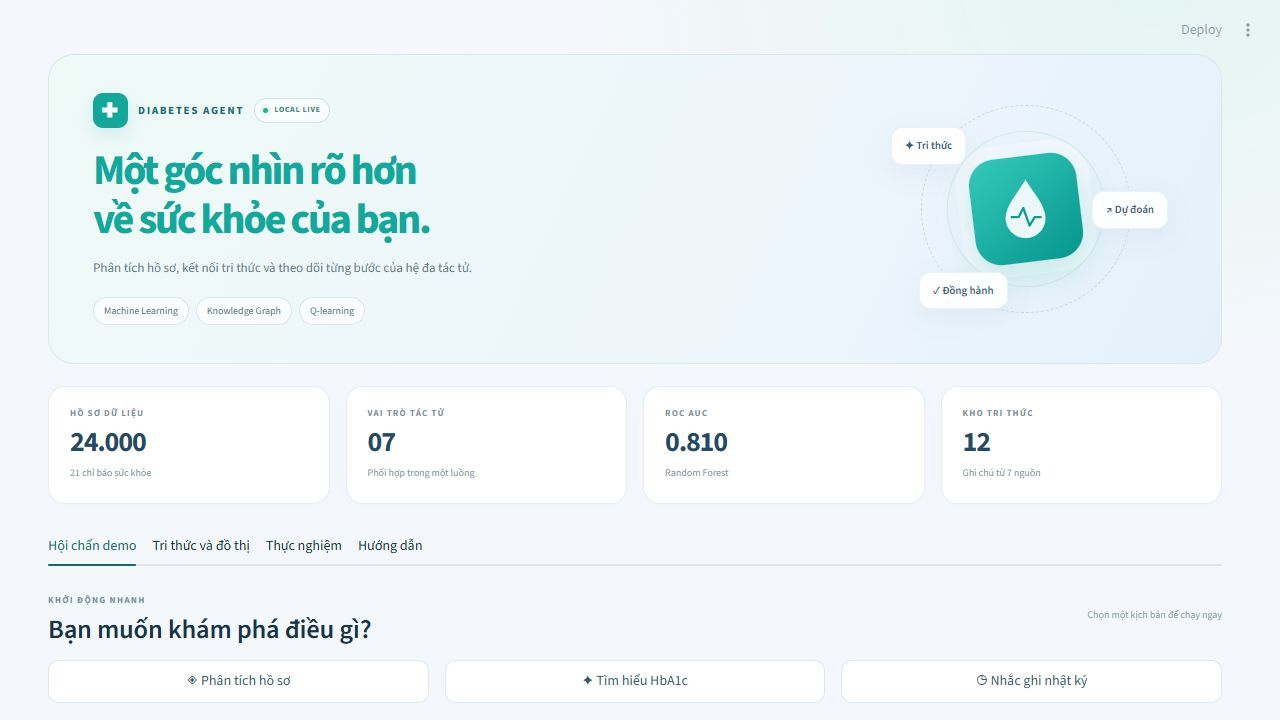
\includegraphics[width=\textwidth]{images/demo_overview.jpg}
\caption{Dashboard tổng quan và các nút chạy nhanh của Diabetes Agent.}\label{fig:demo_overview}
\end{figure}

\clearpage
\section{Kết quả phân loại và phối hợp tác tử}
Ở lượt hội chẩn trong Hình \ref{fig:demo_consult}, Random Forest trả score khoảng 0,147. Với ngưỡng 0,230 đã lưu trong artifact, kết quả thuộc lớp 0. Vòng điểm đi kèm tên mô hình và ngưỡng; các thẻ bên cạnh trình bày tri thức có nguồn và hành động nhắc nhật ký.

Luồng hoàn tất gồm Intake, ba nhánh chuyên môn, Council và Advisor, tạo 12 thông điệp request/response. Bảy thẻ trạng thái phía trên phản ánh các vai trò đã tham gia. Chi tiết phối hợp và nút tải JSON cung cấp proposal, evidence, trạng thái và thời gian xử lý của phiên.
\begin{figure}[H]\centering
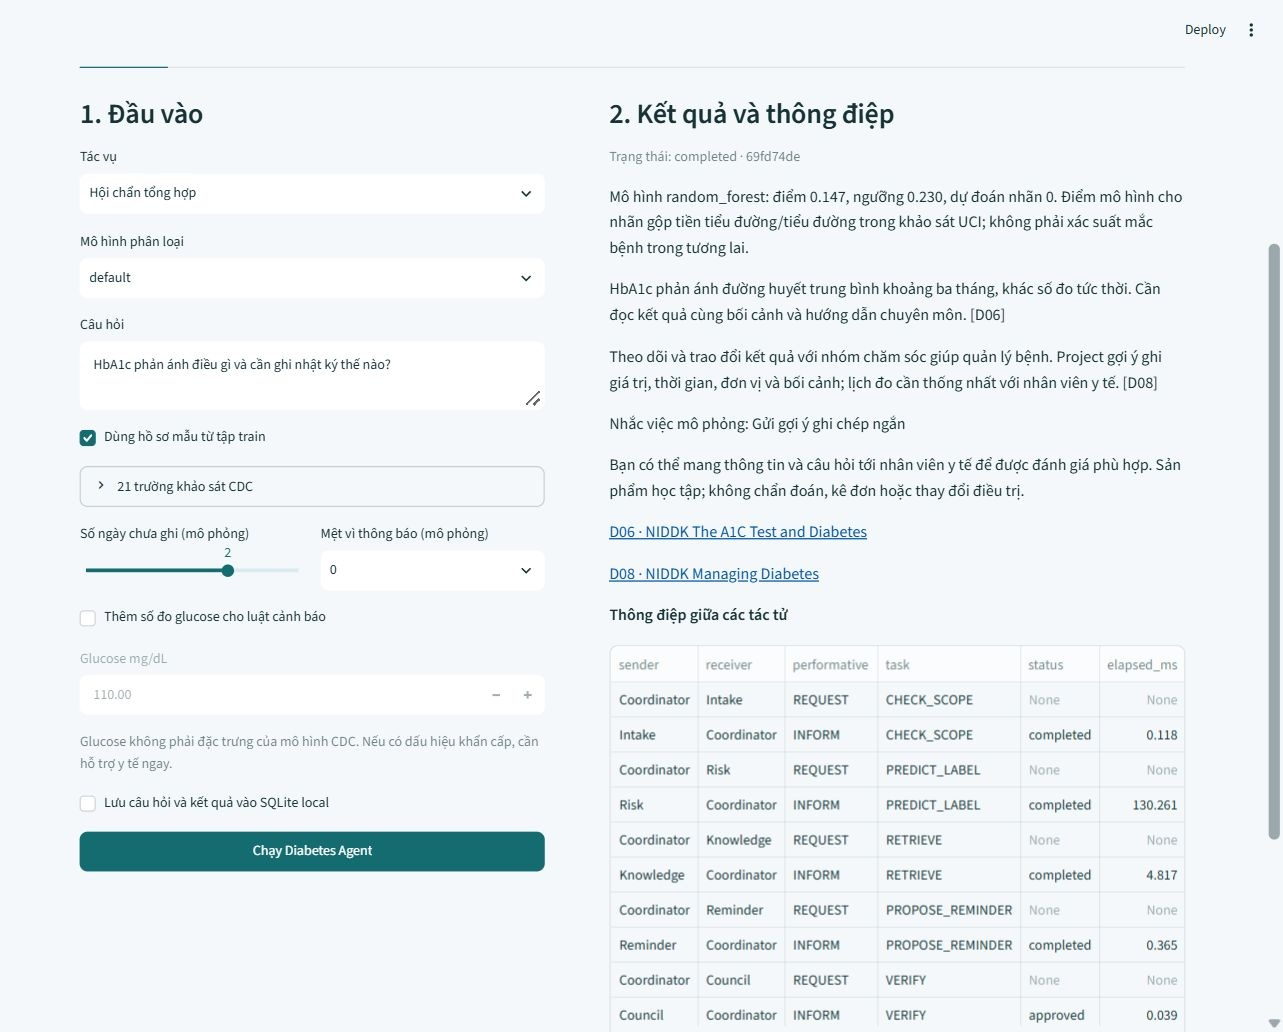
\includegraphics[width=\textwidth]{images/demo_consult.jpg}
\caption{Kết quả hội chẩn với score, ngưỡng phân loại và trạng thái tác tử.}\label{fig:demo_consult}
\end{figure}

\clearpage
\section{Tra cứu tri thức và bản đồ khái niệm}
Truy vấn \emph{HbA1c và thiếu máu} trả các ghi chú D07 và D06 trong ảnh chụp. Mỗi thẻ có ID, nội dung và liên kết nguồn. Bản đồ bên phải biểu diễn quan hệ giữa khái niệm xét nghiệm, HbA1c và các yếu tố ảnh hưởng đến kết quả xét nghiệm.

Tab này cho phép quan sát riêng nhánh Knowledge mà không chạy phân loại hồ sơ hoặc chính sách nhắc việc. Kết quả được lấy từ cùng bộ truy xuất dùng trong lượt hội chẩn.
\begin{figure}[H]\centering
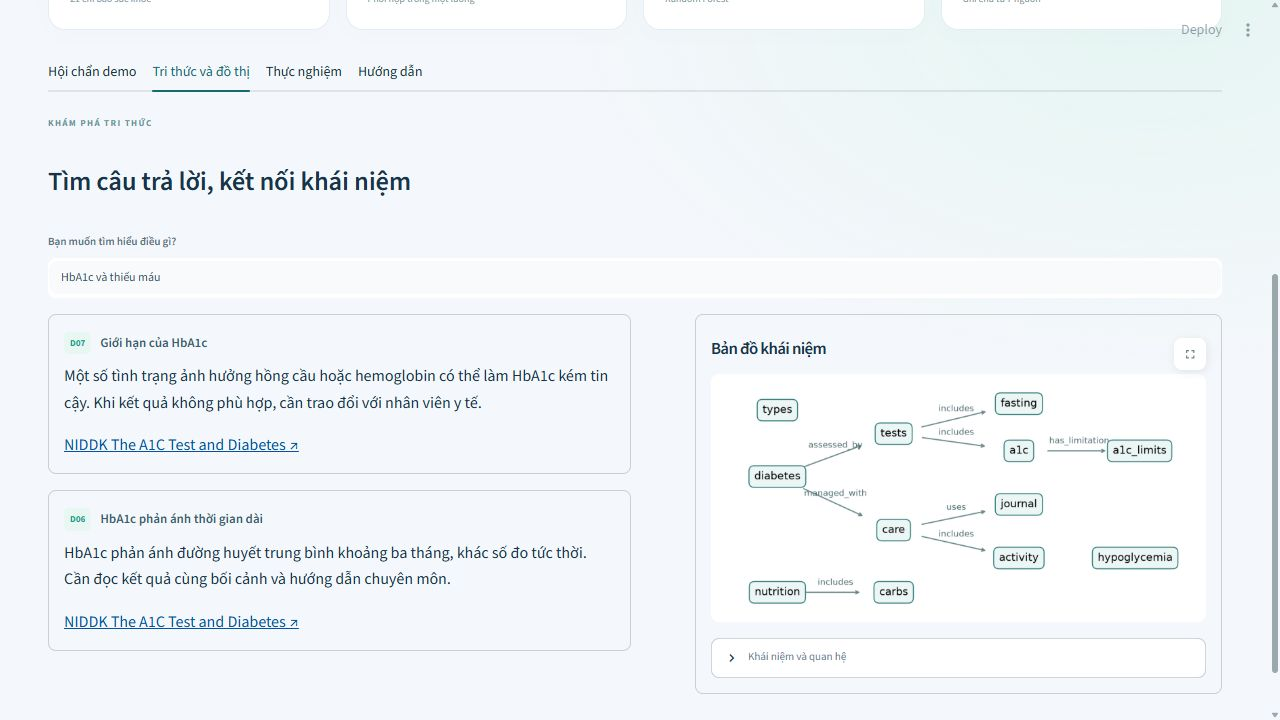
\includegraphics[width=\textwidth]{images/demo_knowledge.jpg}
\caption{Kết quả truy xuất theo câu hỏi và đồ thị khái niệm trên giao diện.}\label{fig:demo_knowledge}
\end{figure}

\clearpage
\section{Biểu đồ thực nghiệm trên giao diện}
Tab Thực nghiệm đọc các bảng đánh giá đã lưu. Bộ chọn chỉ số thay đổi biểu đồ giữa ROC AUC, Average Precision và F1. Với AP test, MLP đạt khoảng 0,3916; Random Forest đạt 0,3906; Logistic Regression đạt 0,3820; Dummy đạt 0,1373.

Biểu đồ nhắc việc hiển thị reward của các policy trong cùng simulator: fixed khoảng 0,2868, Q-learning 0,2703, rule 0,2006 và never 0,0876. Các đường cong và bảng chi tiết phía dưới sử dụng cùng artifact với phần thực nghiệm của báo cáo.
\begin{figure}[H]\centering
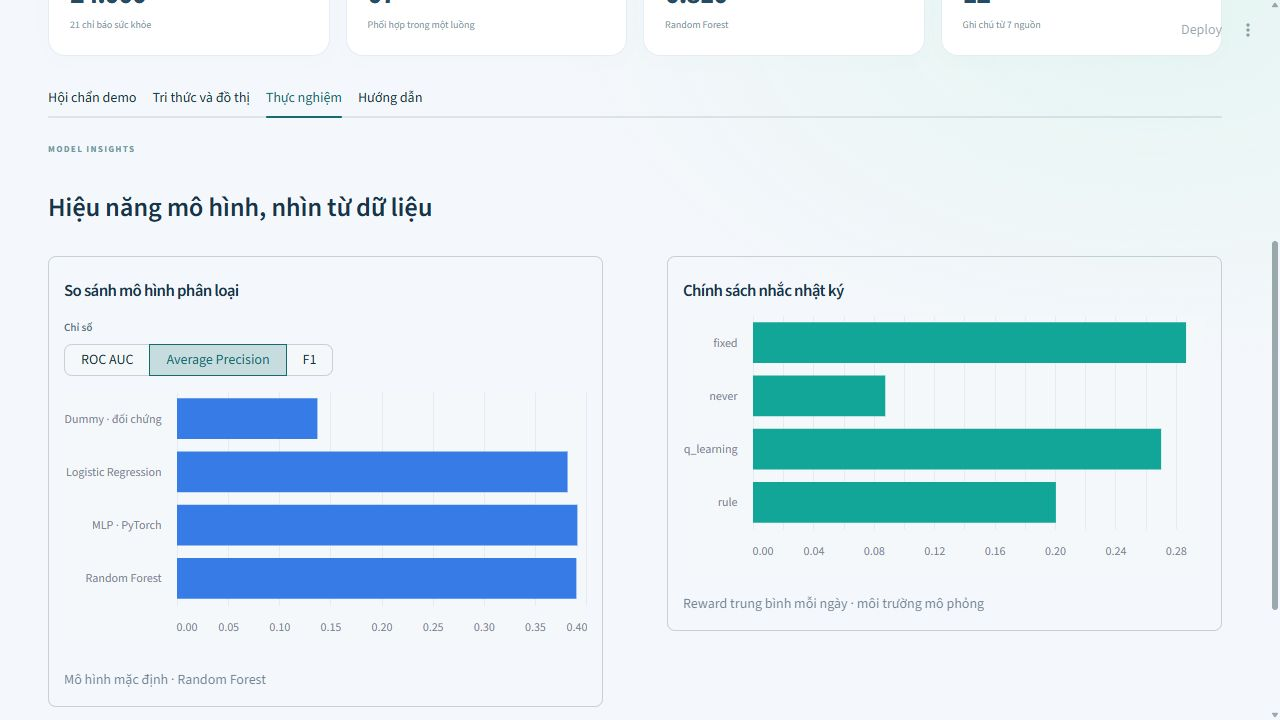
\includegraphics[width=\textwidth]{images/demo_benchmark.jpg}
\caption{Biểu đồ tương tác so sánh mô hình phân loại và chính sách nhắc việc.}\label{fig:demo_benchmark}
\end{figure}

\chapter{Chạy local và trình diễn hệ thống}
\section{Cài đặt môi trường}
Người nhận giải nén toàn bộ thư mục Project01, cài Python 3.11 64-bit và mở terminal tại nơi có \texttt{app.py}. Mô hình, scaler, dữ liệu và KB đã được đóng gói; lần cài đầu chỉ cần tải thư viện. Sau đó demo suy luận có thể hoạt động không cần Internet hoặc API key.

\begin{lstlisting}[language={},caption={Tạo môi trường và khởi động bằng PowerShell.}]
py -3.11 -m venv .venv
.\.venv\Scripts\python.exe -m pip install --upgrade pip
.\.venv\Scripts\python.exe -m pip install torch==2.15.0 --index-url https://download.pytorch.org/whl/cpu
.\.venv\Scripts\python.exe -m pip install -r requirements.txt
.\.venv\Scripts\python.exe -m streamlit run app.py --server.address 127.0.0.1 --server.port 8521
\end{lstlisting}

Mở trình duyệt tại \url{http://127.0.0.1:8521}. Dừng server bằng Ctrl+C trong terminal. Có thể bấm đúp \texttt{run.cmd} để tự tạo môi trường và cài các thư viện ở lần đầu; script cần Python launcher có thể tìm Python 3.11. Nếu dùng Anaconda, tạo env Python 3.11, activate rồi gọi \texttt{python -m pip} và \texttt{python -m streamlit} với cùng tham số.

Gọi trực tiếp Python trong venv giúp tránh lỗi chính sách PowerShell đối với Activate.ps1. Server chỉ bind localhost; project chưa có cấu hình triển khai công khai, đăng nhập hay phân quyền. Khi port 8521 đang được dùng, đổi port và mở đúng URL mới.

\section{Các tab và luồng thao tác}
Giao diện dashboard có bốn tab. Hội chẩn demo có ba nút chạy nhanh, bảy thẻ trạng thái tác tử và vùng thiết lập hồ sơ/câu hỏi. Kết quả chia thành vòng điểm phân loại, các thẻ tri thức và hành động nhắc việc. Tri thức và đồ thị đặt ghi chú có URL cạnh bản đồ khái niệm. Thực nghiệm có biểu đồ tương tác để đổi giữa AUC, Average Precision và F1, cùng bảng/đường cong chi tiết. Hướng dẫn cung cấp các lệnh khởi chạy và tái lập.

Mặc định giao diện dùng hồ sơ mẫu lấy từ train. Người dùng chọn Nhập JSON để thay 21 chỉ báo, chọn tác vụ và bấm Bắt đầu phân tích. Mục Nhật ký và số đo chứa gap, fatigue và glucose bổ sung. Các thẻ tác tử chuyển màu theo thông điệp thực tế của phiên vừa chạy; chi tiết được thu gọn trong mục Chi tiết phối hợp tác tử.

\begin{figure}[H]\centering
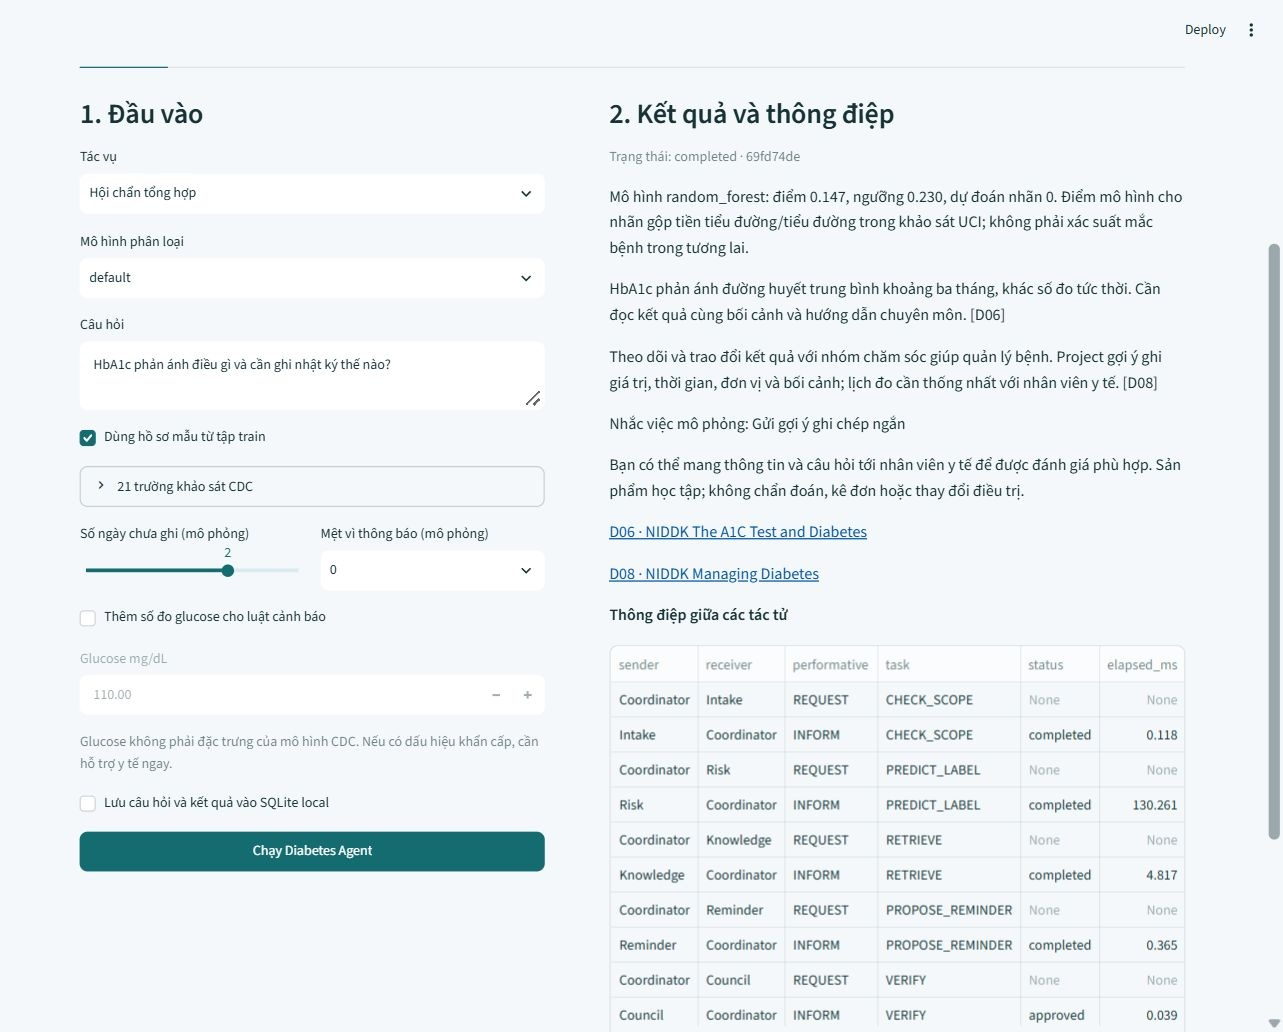
\includegraphics[width=\textwidth]{images/demo_consult.jpg}
\caption{Giao diện local sau khi chạy hội chẩn tổng hợp. Ảnh chụp từ trình duyệt của bản Project01.}
\end{figure}

\section{Ví dụ một lượt hội chẩn}
Với câu hỏi về HbA1c và nhật ký, hồ sơ train minh họa, gap bằng 2 và fatigue bằng 0, hệ thống nhận diện không có điều kiện dừng ở Intake. Risk chạy model mặc định Random Forest, Knowledge truy xuất các ghi chú liên quan và Reminder đọc Q-table seed 42. Council kiểm tra các proposal rồi Advisor ghép kết quả.

Ở hồ sơ minh họa được chọn, score Random Forest khoảng 0,147 và ngưỡng 0,230 nên dự đoán nhãn 0. Giao diện trình bày score bằng vòng điểm, kèm model và ngưỡng. Tri thức được tách thành các thẻ có ID/URL; hành động Reminder nằm trong thẻ nhắc nhật ký. Có thể tải kết quả của cả phiên bằng nút Tải kết quả phiên.

Trace có 12 thông điệp để người đọc thấy thứ tự gọi, trạng thái từng bước và thời gian. Có thể tải JSON để kiểm tra proposal, evidence và lý do duyệt. Bảng trace không phải chuỗi suy nghĩ ẩn của model; nó là log của những thao tác phần mềm thực sự đã gọi.

\begin{figure}[H]\centering
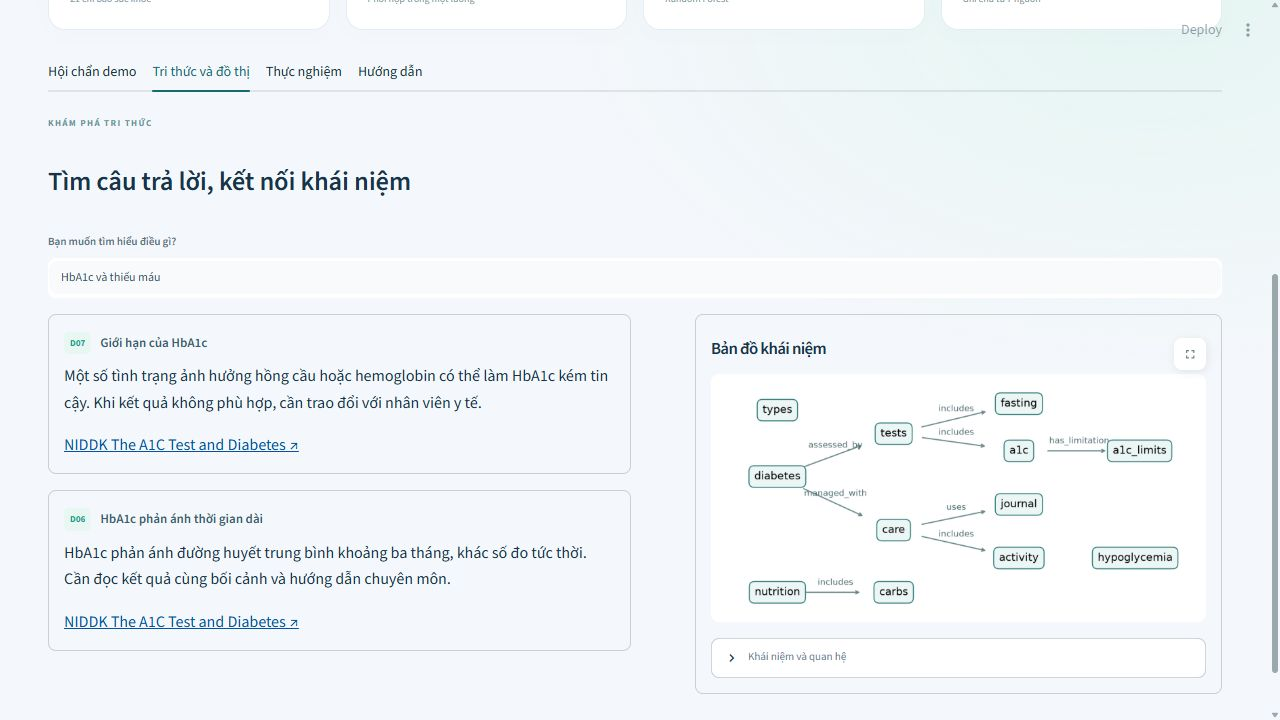
\includegraphics[width=\textwidth]{images/demo_knowledge.jpg}
\caption{Tab tri thức với query, ghi chú và URL nguồn để kiểm tra lại căn cứ.}
\end{figure}

\section{Kịch bản bảo vệ ngắn}
\begin{enumerate}[leftmargin=1.1cm]
\item Giới thiệu ba nhánh học sâu, tri thức và RL; nêu rõ phạm vi giáo dục.
\item Chạy hội chẩn mẫu, chỉ score/ngưỡng, đoạn có ID nguồn, reminder và 12 thông điệp.
\item Chọn riêng MLP; mở notebook 01 để nối từ kiến trúc tới output train và model đã lưu.
\item Hỏi về HbA1c và thiếu máu, mở nguồn của ghi chú; giải thích truy xuất và graph một bước.
\item Nhập hồ sơ chỉ có BMI để cho thấy needs\_input; sau đó thử số đo glucose 62 mg/dL để xem urgent trước Risk.
\item Mở kết quả RL, nêu trung thực Q-learning chưa vượt fixed. Dùng notebook 04 để trình diễn Council bác proposal thuốc hoặc ID giả.
\end{enumerate}
Tài liệu \texttt{docs/KICH\_BAN\_DEMO.md} phân bổ khoảng tám phút cho các thao tác trên. Không dùng hồ sơ thật hoặc nhập thông tin riêng tư khi bảo vệ.

\section{Tái lập thực nghiệm và notebook}
\begin{lstlisting}[language={},caption={Các lệnh tái lập độc lập với giao diện.}]
python scripts/run_experiments.py
python scripts/execute_notebooks.py
python -m pytest -q --junitxml=artifacts/test-results.xml
python scripts/update_report_assets.py
\end{lstlisting}

Các lệnh cần chạy bằng Python của môi trường đã cài dependencies. Script experiment có thể chạy riêng stage models, rl hoặc evaluation. Notebook 01 và 03 train thật nên khi Run All sẽ ghi lại artifact. Không nên mở quá trình train cùng lúc với demo vì app có thể đọc file trong lúc đang ghi. Sau train, khởi động lại app để nạp model mới.

Nếu muốn dùng Jupyter tương tác, chạy \texttt{python -m notebook}, mở theo thứ tự 01--04 và chọn đúng kernel. Mỗi notebook bắt đầu bằng cell in phiên bản Python và xác định thư mục project. Script build\_notebooks chỉ dùng để bảo trì phần source notebook, không tạo output thực và sẽ xóa output cũ nếu chạy lại.

\section{Xử lý lỗi thường gặp}
\begin{table}[H]\centering\small
\caption{Lỗi vận hành và cách xử lý tương ứng.}
\begin{tabularx}{\textwidth}{@{}p{4.1cm}Y@{}}\toprule
Biểu hiện & Cách xử lý \\\midrule
Thiếu module & Cài requirements bằng đúng interpreter chạy app; tránh trộn env Anaconda và venv. \\
Lỗi nạp weight/joblib & Đối chiếu phiên bản đã ghi; dùng env tương thích hoặc huấn luyện lại từ CSV. \\
Thiếu manifest hoặc Q-table & Chạy script experiment trước khi khởi động UI. \\
CSV khác checksum & Khôi phục dữ liệu bàn giao; không sửa checksum chỉ để bỏ kiểm tra. \\
Notebook không tìm thấy module & Mở Jupyter từ Project01 hoặc notebooks trong Project01, kiểm tra cell setup. \\
Score không thay sau train & Dừng và mở lại server để xóa cache resource. \\
Sai mã Age & Dùng nhóm 1--13 theo README dữ liệu; không nhập số tuổi theo năm. \\\bottomrule
\end{tabularx}
\end{table}

\section{Biên dịch lại báo cáo}
Source LaTeX nằm trong \texttt{report/}. Sau khi đổi artifact, chạy script update\_report\_assets để cập nhật bảng và hình đo được. Đọc lại phần diễn giải vì script không tự sửa kết luận trong văn bản. Dùng XeLaTeX hai lượt để cập nhật mục lục, tham chiếu và số trang. README trong thư mục report mô tả các lệnh cụ thể.

\chapter{Kết luận và hướng phát triển}
\section{Kết quả đạt được}
Project01 đã hiện thực một Diabetes Agent chạy local với mã nguồn độc lập, bốn notebook có output thực, dữ liệu có provenance, model đã huấn luyện và giao diện quan sát được quá trình phối hợp.

Kết quả supervised cho thấy các mô hình học được có khả năng phân biệt nhãn trên test nội bộ cao hơn Dummy. Random Forest được chọn mặc định theo AP validation; MLP vẫn được cung cấp và đánh giá đầy đủ. Truy xuất tìm đúng các ID đích trong bộ câu tự xây, còn bộ hợp đồng và pytest xác nhận những nhánh chức năng đã định. Q-learning học được policy có reward hơn never/rule nhưng chưa vượt fixed trong simulator hiện tại.

Giá trị của thiết kế đa tác tử ở project là trách nhiệm được tách rõ, có thông điệp, kiểm tra và quyền từ chối trước khi tổng hợp. Chưa có kết quả chứng minh kiến trúc này tốt hơn một pipeline đơn dùng cùng công cụ. Việc trình bày giới hạn là cần thiết để tách khả năng chạy được của phần mềm khỏi độ tin cậy trong ứng dụng thực.

\section{Giới hạn hiện tại}
Dữ liệu là khảo sát Hoa Kỳ, nhãn gộp và chưa có thẩm định ngoài mẫu. Mã nhóm nhân khẩu được đưa vào dưới dạng số; chưa kiểm tra thiên lệch theo nhóm hoặc phương án mã hóa khác. Supervised mới có một split/seed và chưa có khoảng tin cậy hoặc external validation.

KB nhỏ, bộ câu hỏi tự xây; Council và luật tiếp nhận chỉ kiểm tra các điều kiện đã định. RL dùng reward tự đặt và chưa có dữ liệu hành vi thật. Demo chưa có các yêu cầu vận hành cho hồ sơ bệnh nhân và không thay thế kế hoạch chăm sóc.

\section{Hướng phát triển có thể kiểm chứng}
Bước tiếp theo nên ưu tiên một bộ câu hỏi độc lập và đánh giá thủ công độ liên quan của trích đoạn, trước khi tăng số agent hoặc bổ sung LLM. Với nhánh dự đoán, cần so sánh mã hóa biến, lặp split/seed, báo khoảng bất định, đánh giá calibration và subgroup trong điều kiện sử dụng xác định.

Với RL, cần kiểm tra độ nhạy theo hệ số reward và động lực phản ứng, đối chiếu với nghiệm tối ưu của MDP nhỏ nếu muốn phân tích sai lệch policy. Chỉ chuyển sang nghiên cứu nhắc việc thực tế khi có dữ liệu, đồng thuận và thiết kế đánh giá phù hợp. Những mở rộng này tạo câu hỏi kiểm chứng được, thay vì chỉ tăng độ phức tạp của hệ thống.

\begin{thebibliography}{99}
\addcontentsline{toc}{chapter}{Tài liệu tham khảo}
\bibitem{wooldridge} M. Wooldridge và N. R. Jennings, \textit{Intelligent agents Theory and practice}, The Knowledge Engineering Review, 10(2), 1995. \url{https://www.cs.ox.ac.uk/people/michael.wooldridge/pubs/ker95.pdf}.
\bibitem{watkins} C. J. C. H. Watkins và P. Dayan, \textit{Q-learning}, Machine Learning, 8, 279--292, 1992. \url{https://www.gatsby.ucl.ac.uk/~dayan/papers/cjch.pdf}.
\bibitem{uci} UCI Machine Learning Repository, \textit{CDC Diabetes Health Indicators}, dataset 891, metadata và CSV. \url{https://archive.ics.uci.edu/dataset/891/cdc+diabetes+health+indicators}. Kiểm tra 05/11/2026.
\bibitem{pytorch_bce} PyTorch, \textit{BCEWithLogitsLoss documentation}. \url{https://docs.pytorch.org/docs/stable/generated/torch.nn.BCEWithLogitsLoss.html}. Kiểm tra 05/11/2026.
\bibitem{sklearn_ap} scikit-learn, \textit{average\_precision\_score documentation}. \url{https://scikit-learn.org/stable/modules/generated/sklearn.metrics.average_precision_score.html}. Kiểm tra 05/11/2026.
\bibitem{niddk_basic} NIDDK, \textit{What Is Diabetes}. \url{https://www.niddk.nih.gov/health-information/diabetes/overview/what-is-diabetes}. Kiểm tra 05/11/2026.
\bibitem{niddk_tests} NIDDK, \textit{Diabetes Tests and Diagnosis}. \url{https://www.niddk.nih.gov/health-information/diabetes/overview/tests-diagnosis}. Kiểm tra 05/11/2026.
\bibitem{niddk_a1c} NIDDK, \textit{The A1C Test and Diabetes}. \url{https://www.niddk.nih.gov/health-information/diagnostic-tests/a1c-test}. Kiểm tra 05/11/2026.
\bibitem{niddk_manage} NIDDK, \textit{Managing Diabetes}. \url{https://www.niddk.nih.gov/health-information/diabetes/overview/managing-diabetes}. Kiểm tra 05/11/2026.
\bibitem{cdc_low} CDC, \textit{Treatment of Low Blood Sugar Hypoglycemia}. \url{https://www.cdc.gov/diabetes/treatment/treatment-low-blood-sugar-hypoglycemia.html}. Kiểm tra 05/11/2026.
\bibitem{cdc_food} CDC, \textit{Diabetes Meal Planning}. \url{https://www.cdc.gov/diabetes/healthy-eating/diabetes-meal-planning.html}. Kiểm tra 05/11/2026.
\bibitem{cdc_activity} CDC, \textit{Get Active}. \url{https://www.cdc.gov/diabetes/living-with/physical-activity.html}. Kiểm tra 05/11/2026.
\bibitem{reference_report} Trần Văn Khánh, \textit{Báo cáo Project01 Hệ đa agent hỗ trợ sàng lọc và tư vấn bệnh tiểu đường}, 36 trang, tháng 11/2026.
\end{thebibliography}

\end{document}
